\documentclass[runningheaders,a4paper]{llncs}

\usepackage[ngerman]{babel}
\usepackage{graphicx}
\usepackage[utf8]{inputenc}
\usepackage[T1]{fontenc}
% Darstellung von URLs
\usepackage{url}
\usepackage{amsmath,amssymb}
\usepackage{listings}
\usepackage{subfig}
\usepackage{multirow}
\usepackage{array}
\usepackage{svg}
\usepackage{setspace}
\usepackage{float}
\lstset{language=C++}
\usepackage{float}
\newcommand{\RR}{\mathbb{R}}
\newcommand{\EE}{\mathbb{E}}

\usepackage{tikz}
\usetikzlibrary{calc, arrows,shapes,snakes,automata,backgrounds,petri}
\tikzset{
	%Define standard arrow tip
	>=stealth',
	%Define style for different line styles
	help lines/.style={dashed, thick},
	axis/.style={<->},
	line/.style={thick};
}

\usepackage[]{algorithm2e}
\pagestyle{plain}

\lstdefinelanguage{GLSL}
{
sensitive=true,
morekeywords=[1]{
attribute, const, uniform, varying,
layout, centroid, flat, smooth,
noperspective, break, continue, do,
for, while, switch, case, default, if,
else, in, out, inout, float, int, void,
bool, true, false, invariant, discard,
return, mat2, mat3, mat4, mat2x2, mat2x3,
mat2x4, mat3x2, mat3x3, mat3x4, mat4x2,
mat4x3, mat4x4, vec2, vec3, vec4, ivec2,
ivec3, ivec4, bvec2, bvec3, bvec4, uint,
uvec2, uvec3, uvec4, lowp, mediump, highp,
precision, sampler1D, sampler2D, sampler3D,
samplerCube, sampler1DShadow,
sampler2DShadow, samplerCubeShadow,
sampler1DArray, sampler2DArray,
sampler1DArrayShadow, sampler2DArrayShadow,
isampler1D, isampler2D, isampler3D,
isamplerCube, isampler1DArray,
isampler2DArray, usampler1D, usampler2D,
usampler3D, usamplerCube, usampler1DArray,
usampler2DArray, sampler2DRect,
sampler2DRectShadow, isampler2DRect,
usampler2DRect, samplerBuffer,
isamplerBuffer, usamplerBuffer, sampler2DMS,
isampler2DMS, usampler2DMS,
sampler2DMSArray, isampler2DMSArray,
usampler2DMSArray, struct},
morekeywords=[2]{
radians,degrees,sin,cos,tan,asin,acos,atan,
atan,sinh,cosh,tanh,asinh,acosh,atanh,pow,
exp,log,exp2,log2,sqrt,inversesqrt,abs,sign,
floor,trunc,round,roundEven,ceil,fract,mod,modf,
min,max,clamp,mix,step,smoothstep,isnan,isinf,
floatBitsToInt,floatBitsToUint,intBitsToFloat,
uintBitsToFloat,length,distance,dot,cross,
normalize,faceforward,reflect,refract,
matrixCompMult,outerProduct,transpose,
determinant,inverse,lessThan,lessThanEqual,
greaterThan,greaterThanEqual,equal,notEqual,
any,all,not,textureSize,texture,textureProj,
textureLod,textureOffset,texelFetch,
texelFetchOffset,textureProjOffset,
textureLodOffset,textureProjLod,
textureProjLodOffset,textureGrad,
textureGradOffset,textureProjGrad,
textureProjGradOffset,texture1D,texture1DProj,
texture1DProjLod,texture2D,texture2DProj,
texture2DLod,texture2DProjLod,texture3D,
texture3DProj,texture3DLod,texture3DProjLod,
textureCube,textureCubeLod,shadow1D,shadow2D,
shadow1DProj,shadow2DProj,shadow1DLod,
shadow2DLod,shadow1DProjLod,shadow2DProjLod,
dFdx,dFdy,fwidth,noise1,noise2,noise3,noise4,
EmitVertex,EndPrimitive},
morekeywords=[3]{
gl_VertexID,gl_InstanceID,gl_Position,
gl_PointSize,gl_ClipDistance,gl_PerVertex,
gl_Layer,gl_ClipVertex,gl_FragCoord,
gl_FrontFacing,gl_ClipDistance,gl_FragColor,
gl_FragData,gl_MaxDrawBuffers,gl_FragDepth,
gl_PointCoord,gl_PrimitiveID,
gl_MaxVertexAttribs,gl_MaxVertexUniformComponents,
gl_MaxVaryingFloats,gl_MaxVaryingComponents,
gl_MaxVertexOutputComponents,
gl_MaxGeometryInputComponents,
gl_MaxGeometryOutputComponents,
gl_MaxFragmentInputComponents,
gl_MaxVertexTextureImageUnits,
gl_MaxCombinedTextureImageUnits,
gl_MaxTextureImageUnits,
gl_MaxFragmentUniformComponents,
gl_MaxDrawBuffers,gl_MaxClipDistances,
gl_MaxGeometryTextureImageUnits,
gl_MaxGeometryOutputVertices,
gl_MaxGeometryOutputVertices,
gl_MaxGeometryTotalOutputComponents,
gl_MaxGeometryUniformComponents,
gl_MaxGeometryVaryingComponents,gl_DepthRange},
morecomment=[l]{//},
morecomment=[s]{/*}{*/},
morecomment=[l][keywordstyle4]{\#},
}



\lstset{
backgroundcolor=\color[rgb]{0.95, 0.95, 0.95},
tabsize=2,
rulecolor=,
basicstyle=\scriptsize,
aboveskip={1.5\baselineskip},
columns=fixed,
showstringspaces=false,
extendedchars=true,
breaklines=true,
prebreak = \raisebox{0ex}[0ex][0ex]{\ensuremath{\hookleftarrow}},
frame=single,
showtabs=false,
showspaces=false,
showstringspaces=false,
identifierstyle=\ttfamily,
keywordstyle=\color[rgb]{1.0,0,0},
keywordstyle=[1]\color[rgb]{0,0,0.75},
keywordstyle=[2]\color[rgb]{0.5,0.0,0.0},
keywordstyle=[3]\color[rgb]{0.127,0.427,0.514},
keywordstyle=[4]\color[rgb]{0.4,0.4,0.4},
commentstyle=\color[rgb]{0.133,0.545,0.133},
stringstyle=\color[rgb]{0.639,0.082,0.082},
}

%für pseudocode:
\SetKwProg{Fn}{Function}{}{end}\SetKwFunction{FRecurs}{FnRecursive}%
\SetAlgoLongEnd

% Benötigte Angaben für die Titelseite
\title{ Moment Shadow Mapping, (Moment Based) Volumetric Obscurance und Sample Distribution Shadow Maps }

\author{
	Akasha Jethwa 
	Matrikel-Nr: 2653208
	\and
	Jonas Weinz 
	Matrikel-Nr: 2571421
	\and
	Tom Kneiphof 
	Matrikel-Nr: 2662506
}

% Hier das Institut angeben
\institute{Institut für Informatik der Universität Bonn}

\begin{document}

% Erstellung des Titels
\maketitle

\begin{abstract}
Dieser Bericht ist Teil einer Projektgruppe am Institut für Informatik der Universität Bonn,
die sich mit der Implementierung drei verschiedener Echtzeit-Renderingtechniken für Schatten beschäftigt.
In diesem Bericht wird die Funktionsweise und Implementierung von Sample Distribution Shadow Maps, Volumetric-Obscurance und Moment Shadow Mapping behandelt.
Alle drei Techniken werden in einer kleinen Engine implementiert und in einem Demo-Spiel verwendet.
\end{abstract}


\section{Einleitung}
Das Rendern von Schatten ist ein wichtiger Aspekt der interaktiven 3D Grafik.
Die Struktur einer Szene wirkt durch Schatten realisitischer und hilft dem Betrachter dabei, Relationen zwischen Objekten besser zu verstehen.
Allerdings ist das Berechnen der verschiedenen Schattentechniken aufwendig und oft anfällig für Artefakte.
Deshalb untersuchen wir in diesem Paper 3 Techniken, welche verschiedene Lösungsansätze und Vorteile bieten.
Zusätzlich implementieren wir alles in einer eigenen 3D Engine und generieren daraus ein kurzes Spiel um die Techniken zu demonstrieren.


% Introduction
\subsection{Sample Distribution Shadow Maps}

Ein häufiges Problem bei der Shadow Map Generierung ist Aliasing durch Over und Under Sampling.
Sample Distribution Shadow Maps (SDSMs) \cite{sdsm} sind ein voll automatisches Verfahren mit konstantem Speicherbedarf und einer vorhersagbaren Worst-Case Laufzeit, die nicht von der Szenenkomplexität abhängt.
Das Verfahren ist dadurch sehr gut für den Einsatz in Echtzeit Grafikanwendungen geeignet.
SDSM ist ein Screen Space Verfahren, welches adaptiv in jedem Frame Z-Partitionen \cite{zpart} (Hier auch Kaskaden \cite{csm}) erstellt.
So wird mehr Shadow Map Auflösung für Bereiche in der Nähe der Kamera zur Verfügung gestellt und weniger für weit entfernte Bereiche, wodurch perspektivischem Aliasing entgegen gewirkt wird.
Des Weiteren werden die Shadow Map Frusta von SDSMs eng um die tatsächlich sichtbare Geometrie gelegt, was die zur Verfügung stehende Auflösung in den Shadow Maps zusätzlich erhöht.


% Introduction
\subsection{Volumetric Obscurance}
Obscurance (= Umgebungsverdeckung) ist eine Technik zur Berechnung von Schatten basierend auf der Annahme,
dass sich gegenseitig verdeckende Geometrie zu einem verringerten Lichteinfall führt.
In diesem Paper werden wir verschiedene Screenspace-Algorithen für Volumetric Obscurance erläutern und kurz unsere Implementationen vorstellen.


% Introduction
\subsection{Moment Shadow Mapping}
Wir wollen filterbare Schatten verwenden, die eine möglichst hohe Qualität liefern und dabei performant bleiben.\\
Moment Shadow Mapping (MSM) liefert uns dieses Verfahren und wird im weiteren Verlauf erläutert und implementiert. Dieses Verfahren ähnelt den Variance Shadow Maps und ermöglicht ein Filtern und Anti-Aliasing durch speichern zusätzlicher Informationen und nutzen einer 4-Kanal Textur.\\MSM bietet uns eine effiziente Heuristik für gefilterte Hardshadows. Desweiteren werden Light-Leaking Artefakte gemindert und ein realistisches Bild für Schatten geliefert.\\
Zusätzlich betrachen wir Moment Based Volumetric Obscurance (MBVO) welcher auf der MSM Technik basiert.

\section{Related Work}

% Related Work
\subsection{Sample Distribution Shadow Maps}

Parallel Split Shadow Maps (PSSMs) \cite{pssm} ist ein existierendes Verfahren um perspektivisches Aliasing zu minimieren.
Allerdings liefert es nicht immer gute Ergebnisse und hängt von Parametern ab, deren optimaler Wert unbekannt ist und oft von der betrachteten Szene abhängt.

Andere Verfahren wie Adaptive Shadow Maps \cite{asm} und Resolution-Matched Shadow Maps \cite{rmsm} verwalten eine komplexe Baumstruktur von Shadow Maps um die Shadow Map Auflösung adaptiv in der Szene zu verteilen.
Sie erreichen eine hohe Qualität auf Kosten von Performanz, wodurch sie für Echtzeitanwendungen eher ungeeignet sind.

The Irregular Z-Buffer \cite{irregular} ist ein Verfahren, das die Shadow Map an willkürlichen Punkten abtastet.
Dadurch werden Aliasing Effekte gänzlich vermieden.
Allerdings ist das Verfahren nicht oder nur schlecht auf heutigen GPU's implementierbar und läuft nur sehr langsam auf CPU's, wodurch es für das Echtzeit Rendering nicht geeignet ist.


% Related Work
\subsection{Volumetric Obscurance}

Ambient Occlusion (= Umgebungsverdeckung) ist eine Rendertechnik um Schatten in 3D-Szenen
zu approximieren. Dafür gibt es allgemein 2 Ansätze:
\begin{enumerate}
	\item "Global Illumination Based Ambient Occlusion": für jeden Punkt in der Szene wird geprüft, ob der Himmel von diesem
		Punkt aus sichtbar ist (bzw. bei geschlossenen Szenen: ob eine maximale Distanz ohne Kollision erreicht
		 werden kann). Dieses Verfahren ist relativ teuer, kann aber z.B. für statische Szenen vorberechnet
		 werden. (Abb. \ref{ref:aoImage})
		\cite{aoPaper}
	\item Screenspace Ambient Occlusion (SSAO): Es wird der Tiefenbuffer im Screenspace betrachtet. Für jeden Pixel innerhalb einer Umgebung wird die Verteilung im Tiefenbuffer evaluiert und anhand der Differenzen
	ein Schattierungsfaktor berechnet. (Abb. \ref{ref:ssaoImage})  \cite{cry2Paper}
\end{enumerate}  

\begin{figure}[H]
	\centering
	\subfloat[Global Illumination Based Ambient Occlusion]{
		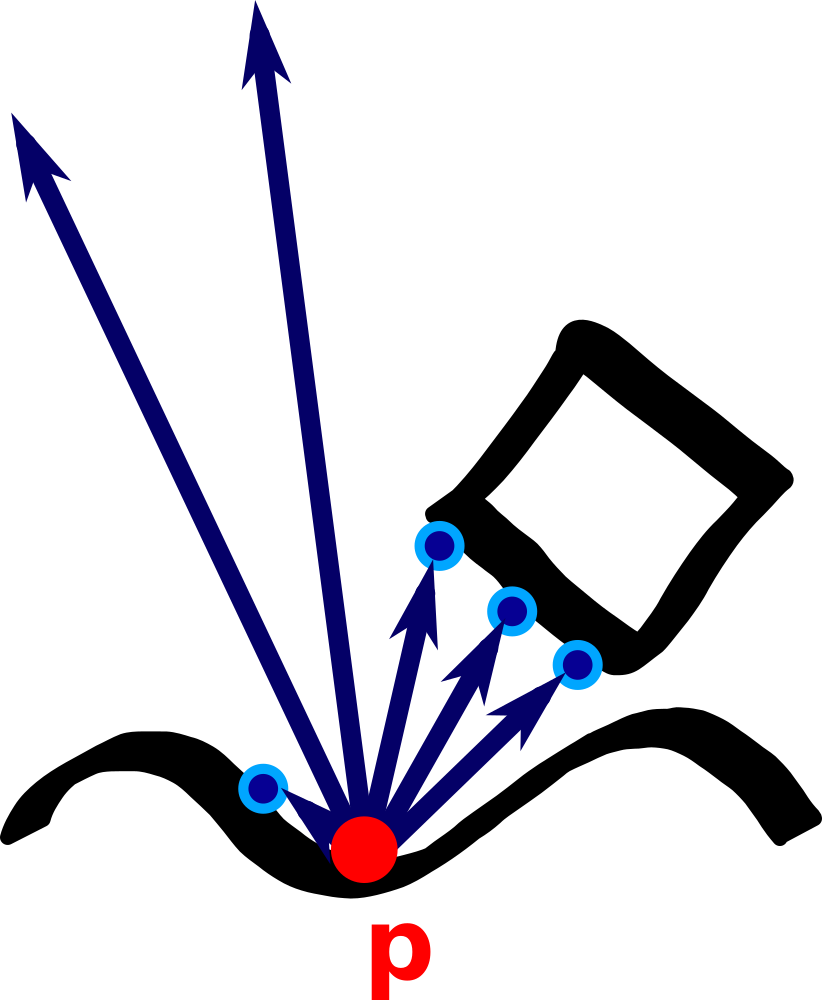
\includegraphics[width=3cm]{vo_assets/aoScematic.png}
		\label{ref:aoImage}
	}\quad \quad
	\subfloat[Screenspace Ambient Occlusion]{
		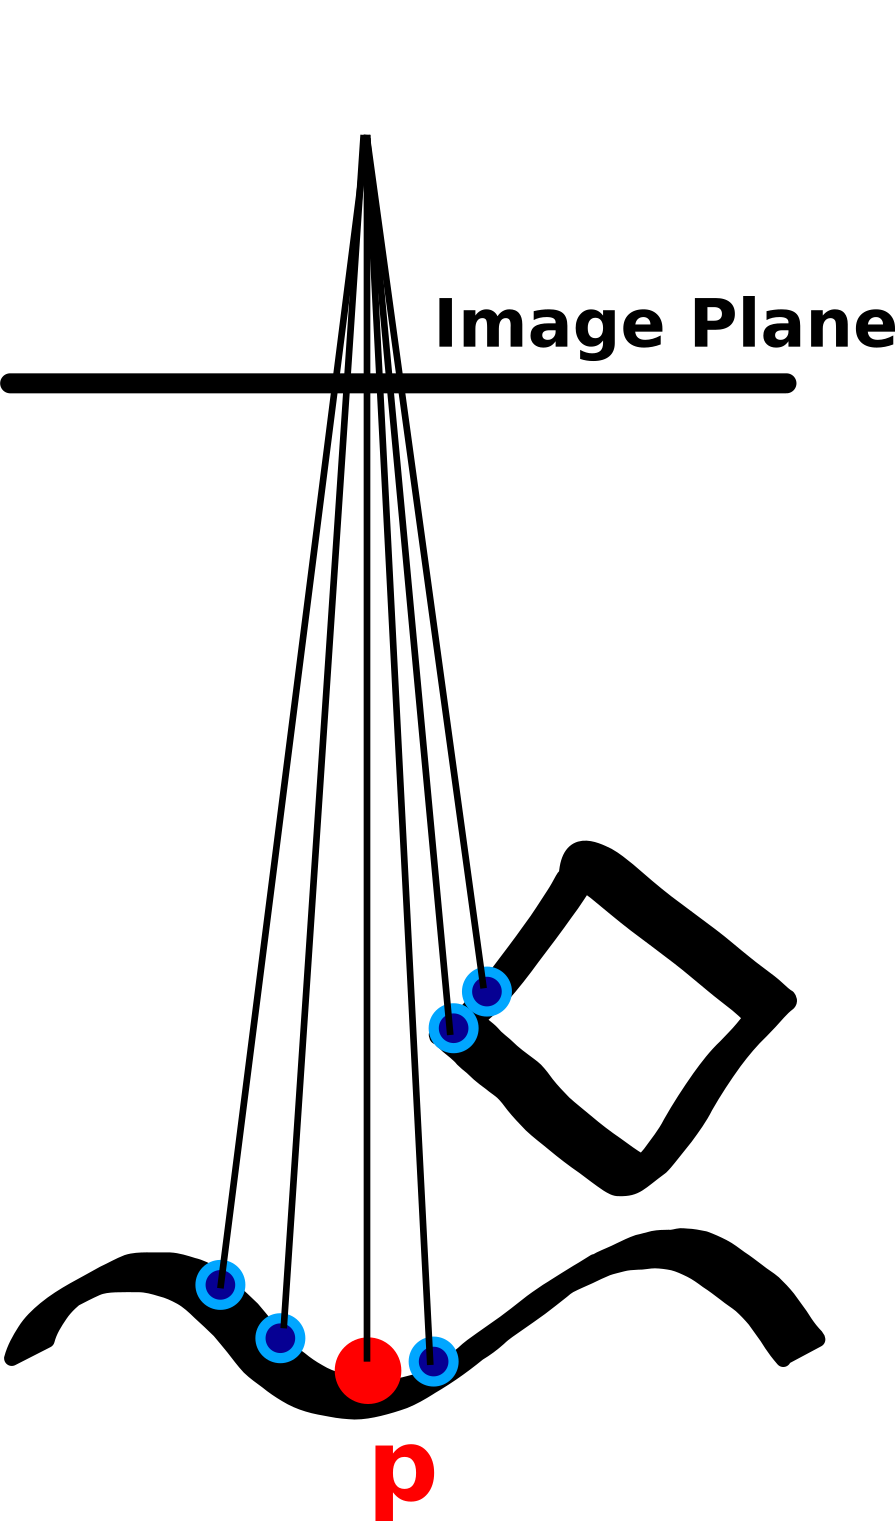
\includegraphics[width=3cm]{vo_assets/ssaoSchematic.png}
		\label{ref:ssaoImage}
	}\quad \quad
	\subfloat[Volumetric Obscurance]{
	    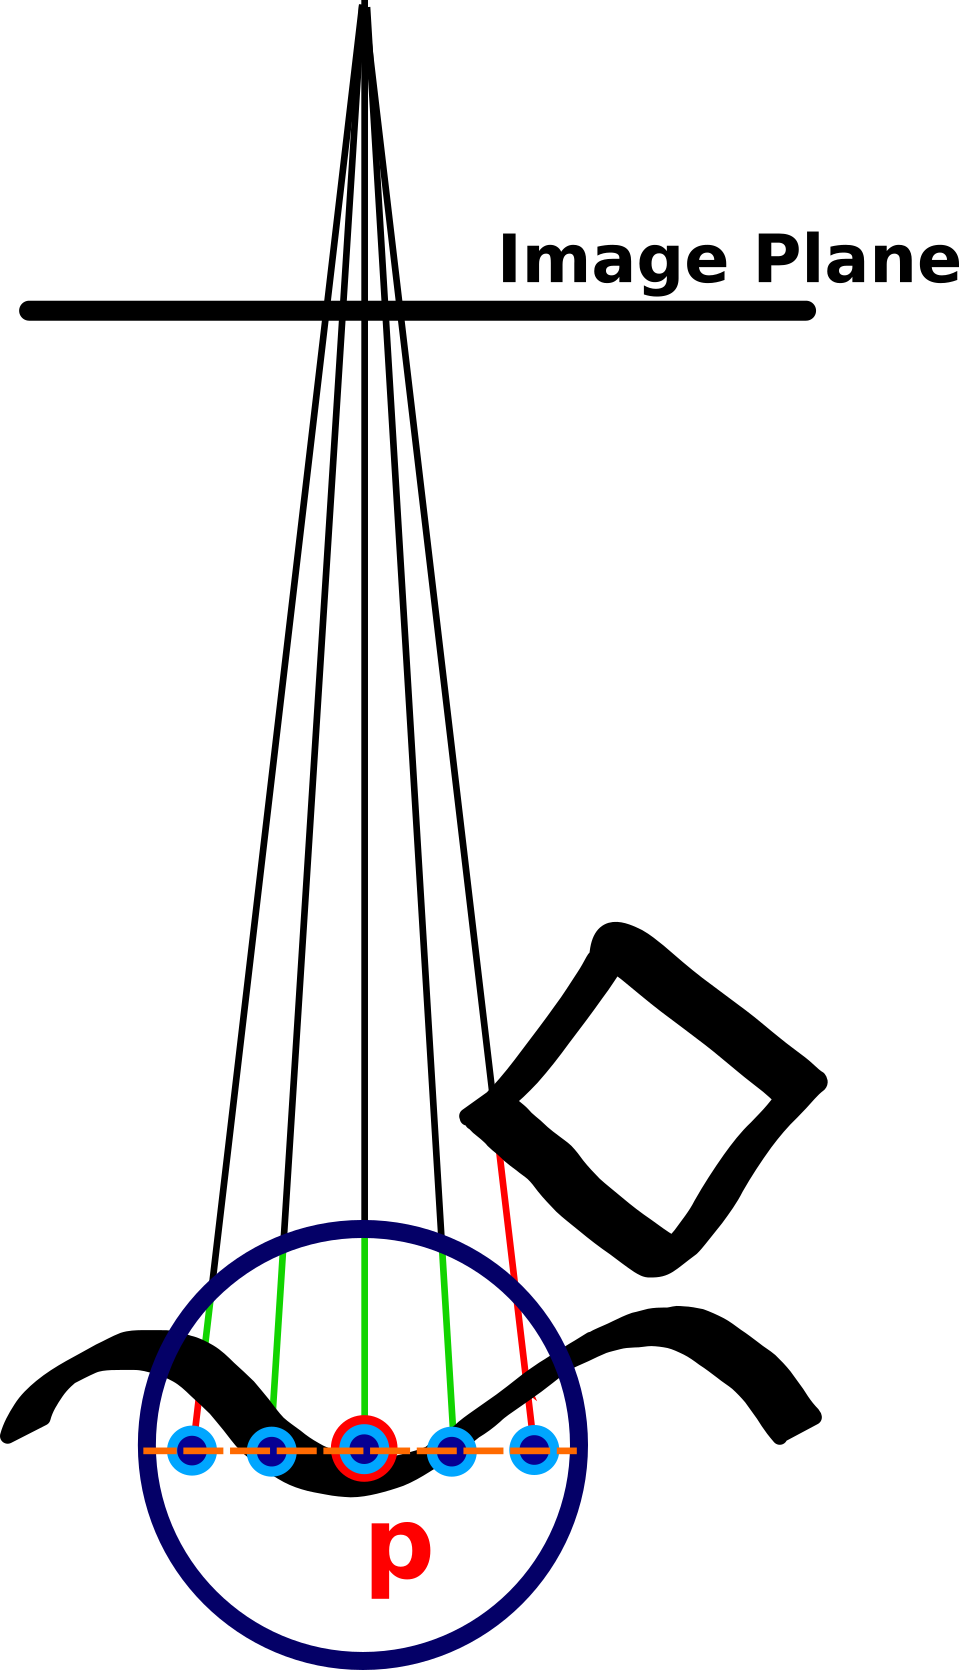
\includegraphics[width=3cm]{vo_assets/voSchematic.png}
		\label{ref:voImage}
	}
	\caption{
		Umgebungsverdeckungstechnicken im Vergleich
	}
\end{figure}

Volumetric Obscurance (Abb. \ref{ref:voImage}) ist eine Alternative zum Screenspace Volumetric Obscurance, welche wir im folgenden
Erläutern werden

\cite{voPaper}

% Related Work
\subsection{Moment Shadow Mapping}
%NEUER TEIL
Grundsätzlich behandel wir Themen des Shadow Mapping um Echtzeit-Schatten zu berechnen. Dies bedeutet, dass wir eine Szene aus Sicht des Lichtes rendern. Wir nutzen die Szenentiefe als Information und speichern diese. Dadurch sind wir in der Lage belichtete Flächen durch ihre Sichtbarkeit zu beschreiben. Der Vorteil ist, dass dieses Verfahren auf der Hardware implementiert ist und deswegen performant genutzt werden kann. Nachteilig ist das sogenannte Aliasing durch Undersampling, also unschöne Artefakte, welche im z.B. in Randbereichen von Objekten und deren Schatten auftreten.\\
Shadow Maps können nicht direkt gefiltert werden um diese Artefakte zu vermeiden. Wir möchten im weiteren Verlauf Verfahren finden, die dies ermöglichen um die Vorteile des Filterns und Anti-Aliasing zu nutzen.\\
Ein erster Ansatz hierfür ist Percentage Closer Filtering (PCF). Jeder Texel der Shadow Map liefert uns eine tiefenabhängige Schattenintensität für den zugehörigen Light Ray. Dadurch können belichtete Flächen erkannt werden, welche vor dem zugehörigen Tiefenwert liegen, also kleiner sind bzw. Flächenwerte nach diesem Tiefenwert liegen im Schatten, sind also größer als jene Tiefe.\\
Mit Hilfe dieser Informationen können gewichtete Kombinationen der Funktionen, mit Gewichten eines Filter Kernels, erstellt werden. Dies liefert uns die Tiefenabhängige Schattenintensität für das Percentage Closer Filtering. \cite{reeves1987rendering}\\
Dies kann als eine Wahrscheinlichkeitsfunktion $z$ interpretiert werden. $z$ sagt uns, wie wahrscheinlich es ist, dass ein Sample des Kernels kleiner als die abhängige Tiefe ist. Ziel ist es, diese Funktion vorher zu berechnen, da dies nicht direkt in der Shadow Map möglich ist.\\
Dies wiederrum, führt uns zu den Variance Shadow Maps (VSM), welche nicht nur die Tiefe $z$, sondern auch $z^2$ in einer 2 Kanal Textur speichern. Diese, zunächst reduntante Information, kann nun zum Filtern und Anti-Aliasing genutzt werden. Dies wird deswegen ermöglicht, da wir durch die so gefilterten Vektoren der Variance Shadow Map, eine Rekonstruktion der tiefenabhängigen Schattenintensität ermöglichen.\cite{donnelly2006variance}\\ Dies ist bereits sehr effizient und mindert die Aliasing-Artefakte. Allerdings ist VSM weiterhin anfällig für Light-Leaking.\\
Desweiteren können die ungefilterten Texel als Punkte in einer Parabel gesehen werden. Dies bedeutet, dass verschiedene Texel, verschiedene Punkte speichern. Dach dem Filtern, können diese Vektoren allerdings als Massezentrum jener Punkte, welche betrachtet wurden, verstanden werden. Diese, nicht länger redundante Information, gibt uns bereits Wissen über die Tiefenfunktion, da wir einen Erwartungswert von $z$ und $z^2$ interpretieren könnem welcher abhängig von der Tiefe ist. Diese werden auch Momente der Tiefenfunktion genannt und bereits 2 Momente ermöglichen uns eine Rekonstruktion und Approximierung der Tiefenfunktion. Vorteilhaft ist ebenfalls, das diese immer die Schattenintensität unterschätzt, also eine untere Schranke bildet. Algorithmisch ist die Rekonstrukion mit Chebyshev's Ungleichung möglich. \cite{donnelly2006variance}


% Main
\section{Sample Distribution Shadow Maps}

Sample Distribution Shadow Maps (SDSMs) ist ein Verfahren zur adaptiven Optimierung der Shadow Map Auflösung unter Verwendung des Camera-Space Depth Buffers.

% SDSM
\subsection{Algorithmus}

% Cascaded Shadow Maps aka Z-Partitioning
SDSMs basieren auf Z-Partitoning, wobei das Kamera Frustum entlang der Blickrichtung in mehrere Kaskaden partitioniert wird.
Für jedes Kaskade wird eine eigene Shadow Map generiert.
Auf diese Weise kann mehr Shadow Map Auflösung für nahe Objekte verwendet werden, und weniger Auflösung für weit entfernte Objekte.


% Betrachte Punkte in Light-Space TODO
Der Algorithmus betrachtet die Verteilung aller sichtbaren Punkte der Szene aus der Sicht des Lichtes (im Light-Space).
Hierzu wird für jedes Sample aus dem Camera-Space Depth Buffer die Position in der Welt rekonstruiert und in den Light-Space transformiert.
Die so erhaltenen Punkte sind genau die Punkte, für die beim Rendern der Szene aus der Sicht der Kamera auf die Shadow Map zugegriffen wird.


% Partitionierung
Für gute Ergebnisse ist eine geeignete Wahl der Partition ausschlaggebend.
Anstatt auf eine statische Partitionierung des Kamera Frustums \cite{pssm} zu setzen, wird die Partitionierung von SDSMs in jedem Frame neu berechnet, so dass sie die sichtbare Geometrie optimal abdeckt.

% - Min/Max Reduktion
% - Logarithmische Partitionierung
Zunächst wird die tatsächliche Near und Far Distanz der sichtbaren Geometrie im Kamera Frustum ermittelt.
Dies geschieht mittels Min/Max Reduktion der Tiefenwerte im Camera-Space Depth Buffer.
Anschließend wird das Kamera Frustum zwischen tatsächlicher Near und Far Distanz logarithmisch partitioniert um das perspektivische Aliasing zu minimieren.


% SDSM Cascades colorized
\begin{figure}[H]
	\centering
	\subfloat{
		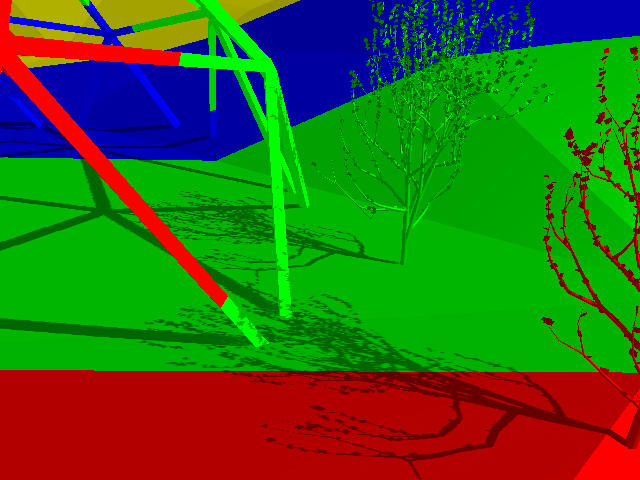
\includegraphics[width=5.5cm]{sdsm_assets/pssm_colorized_near.png}
	}
	\subfloat{
		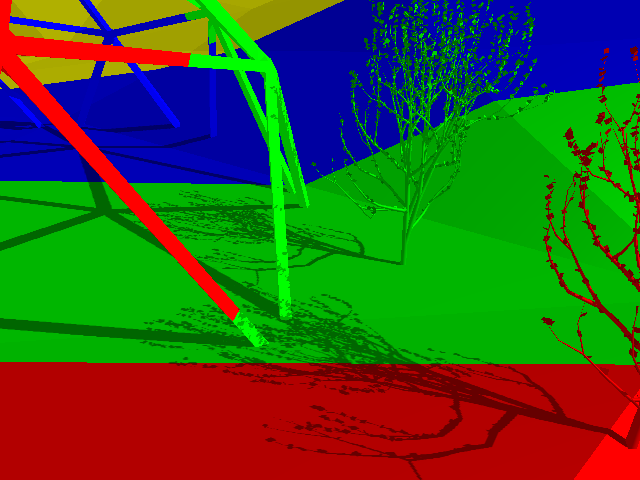
\includegraphics[width=5.5cm]{sdsm_assets/sdsm_colorized_near.png}
	}
	
	\subfloat{
		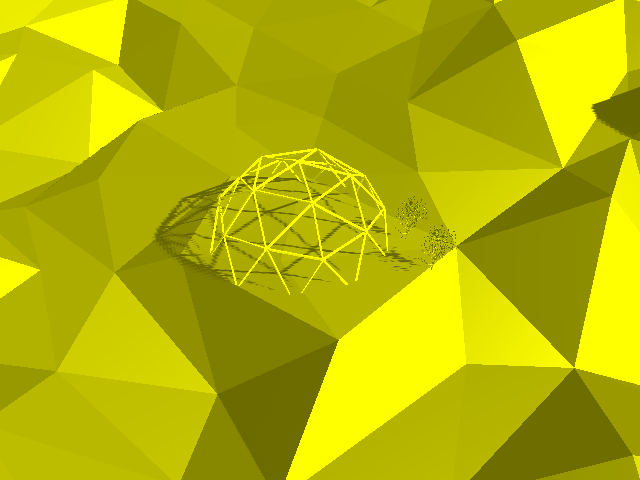
\includegraphics[width=5.5cm]{sdsm_assets/pssm_colorized_far.png}
	}
	\subfloat{
		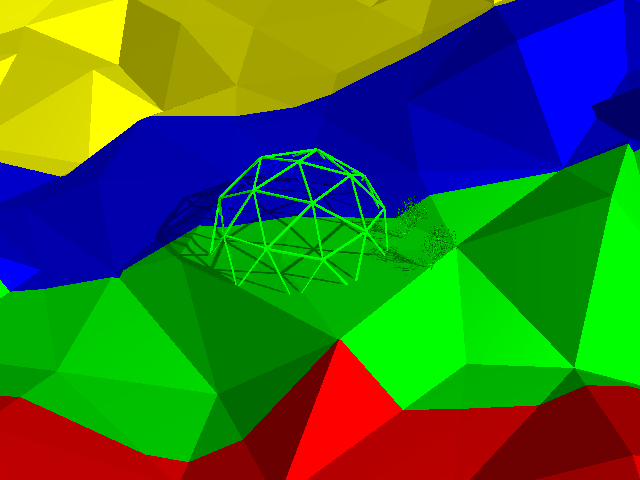
\includegraphics[width=5.5cm]{sdsm_assets/sdsm_colorized_far.png}
	}
	
	\caption{
		Visualisierung der Kaskaden in den Farben rot (nah), grün, blau, gelb (fern).
		Links sind Partitionierungen durch Parallel Split Shadow Maps zu sehen.
		Rechts sind Partitionierungen durch Sample Distribution Shadow Maps zu sehen.
		Die Partitionierung der PSSMs ist für das obere linke Bild optimiert.
		Während SDSMs die Kaskaden unten rechts adaptiv anpassen können, versagen die PSSMs in dem unteren linken Bild und.
	}
\end{figure}


% Abgrenzung PSSM Logarithmic/Linear
PSSMs kennen die tatsächliche Near und Far Distanz nicht, und müssen mit der Near und Far Distanz der Projektionsmatrix arbeiten.
Eine logarithmische Partitionierung würde zu viel Shadow Map Auflösung in den sehr nahen Bereich verschieben, der oft leer ist.
PSSMs konvexkombinieren die Partitionsgrenzen der linearen und logarithmischen Partitionierung um mehr Auflösung von der Near Plane weg zu bewegen.
Optimale Koeffizienten müssen meist von Hand ermittelt werden und sind nicht universell gültig.

% (K-Means and friends)
Weitere Möglichkeiten das Kamera Frustum intelligent zu partitionieren, sind ein adaptiv logarithmisches und ein K-Means Verfahren.
Das adaptiv logarithmische Verfahren vermeidet Lücken im Histogramm des Kamera Depth Buffers, indem es die Partitionsgrenzen an das Ende von diesen schiebt.
Das K-Means Verfahren sucht zunächst Maxima im Histogramm des Kamera Depth Buffers und legt dann die Partition entsprechend um die gefundenen Maxima.
Für beide Verfahren muss zunächst das Histogramm des Camera Depth Buffers berechnet werden.


% Tight Partition Frusta
Andere Algorithmen wie PSSM \cite{pssm} projizieren die Ecken des Kamera Frustums bzw. der Kaskaden in den Light=Space um das Frustum für die Shadow Map zu erhalten.
Um das Frustum möglichst klein zu wählen, kann dort eine Oriented Bounding Box anstelle einer Axis Aligned Bounding Box (AABB) berechnet werden.
Die Konvexe Hülle der in den Light-Space projizierten Punkte kann ein sehr komplexes Polygon werden, weshalb es sich für SDSMs nicht lohnt diese zu berechnen.

SDSMs berechnen für jede Kaskade eine AABB, die dann das Frustum für die Shadow Map bildet.
Damit die AABBs die sichtbare Geometrie sinnvoll umschließen, wird der Light-Space so rotiert, dass die Z-Achse des Camera-Spaces sich an der X-Achse des Light-Spaces ausrichtet.


% SDSM Camera View
\begin{figure}[H]
	\centering
	\subfloat[PSSM] {
		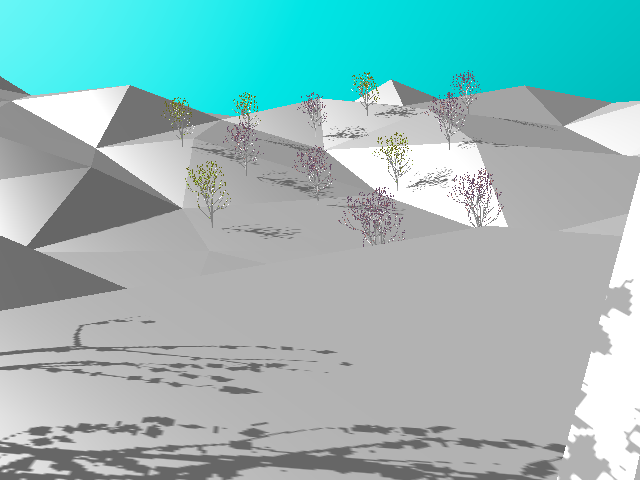
\includegraphics[width=5.5cm]{sdsm_assets/sdsm_pssm_comparision_2/pssm_scene_small.png}
	}
	\subfloat[SDSM] {
		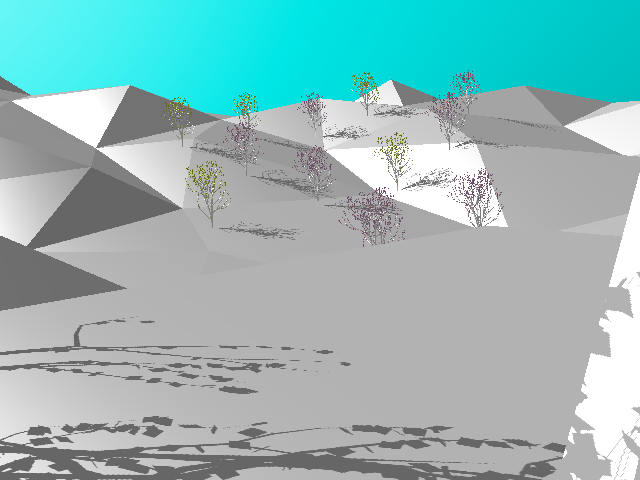
\includegraphics[width=5.5cm]{sdsm_assets/sdsm_pssm_comparision_2/sdsm_scene_small.png}
	}

	\subfloat[PSSM] {
		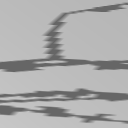
\includegraphics[width=2.5cm]{sdsm_assets/sdsm_pssm_comparision_2/pssm_area0.png}
	}
	\subfloat[SDSM] {
		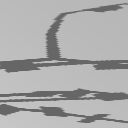
\includegraphics[width=2.5cm]{sdsm_assets/sdsm_pssm_comparision_2/sdsm_area0.png}
	}
	\qquad
	\subfloat[PSSM] {
		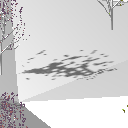
\includegraphics[width=2.5cm]{sdsm_assets/sdsm_pssm_comparision_2/pssm_area1.png}
	}
	\subfloat[SDSM] {
		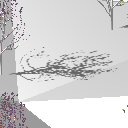
\includegraphics[width=2.5cm]{sdsm_assets/sdsm_pssm_comparision_2/sdsm_area1.png}
	}
	
	\caption{Eine Szene die weit entfernte und sehr nahe Schatten enthält.}
\end{figure}

%  SDSM Light View
\begin{figure}[H]
	\centering
	\subfloat[PSSM] {
		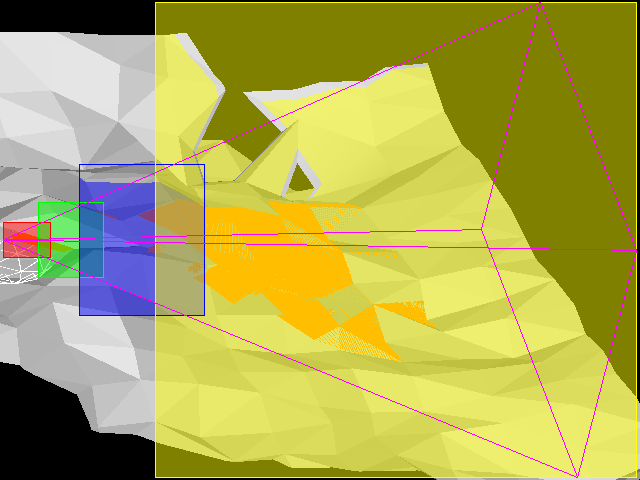
\includegraphics[width=5.5cm]{sdsm_assets/sdsm_pssm_comparision_2/pssm_light_view_small.png}
		\label{ref:pssm_light}
	}
	\subfloat[SDSM] {
		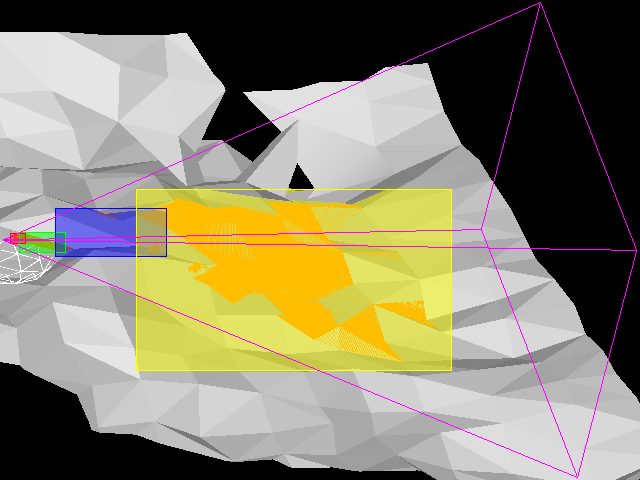
\includegraphics[width=5.5cm]{sdsm_assets/sdsm_pssm_comparision_2/sdsm_light_view_small.png}
		\label{ref:sdsm_light}
	}

	\caption{Visulaisierung der von den Shadow Maps abgedeckten Bereiche mit PSSM und SDSM im Light-Space.}
\end{figure}



% SDSM
\subsection{Implementierung}

% Rendern der Shadow Map
Die Shadow Maps für die Kaskaden werden mittels Texture Arrays realisiert, wobei jede Kaskade einen eigenen Layer in dem Array erhält.
Beim Rendern der Shadow Map transformiert der Vertex Shader die Geometrie zunächst nur in den World-Space und nicht direkt in das Frustum der Shadow Map.
Der Geometry Shader klont dann die Geometrie und transformiert sie für jede Kaskade mit der dazugehörigen Projektionsmatrix in das Shadow Map Frustum um sie in den entsprechenden Layer der Shadow Map zu rendern.
Anstatt die Near Plane des Shadow Map Frustums zu verschieben, um Geometrie die aus der Sicht des Lichtes vor dem Camera Frustum liegt zu berücksichtigen, wird an der Near Plane des Shadow Map Frustums der Tiefenwert geclampt.

% Temporäre Licht Projektion
Um die Bounding Boxen der Geometrie in den einzelnen Kaskaden zu berechnen, müssen die Koordinaten im Light-Space auf den Bereich $[0, 1]$ gemappt werden.
Hierzu werden die Eckpunkte des Screen-Spaces in die Welt, und anschließend in den Light-Space transformiert, wo dann deren Axis Aligned Bounding Box auf $[0, 1]^3$ projiziert wird.
So ist es garantiert, dass die Koordinaten sämtlicher sichtbarer Geometrie im Light-Space ohne clamping in einer Textur gespeichert werden können.

% Reduktion 1 & 2
Die beiden Reduktionen werden jeweils in einem Compute Shader ausgeführt.
Jeder Thread liest 1 bis 4 Einträge pro zu reduzierendem Wert ein.
Jede Thread Gruppe (von 256 Threads) generiert einen neuen Eintrag pro Wert.
Ausserdem versuchen wir die Zugriffsmuster auf den Shared Memory so weit es geht zu optimieren und Bank Conflicts zu vermeiden \cite{reduction}.
Um so mehr verschiedene Werte auf einmal reduziert werden, desto mehr können idle Zeiten von Threads in den Thread Gruppen vermieden werden.

Anstatt nach einer halbierung der Daten die eine Hälfte der Threads ihre Arbeit beendigen zu lassen, wird der erste zu reduzierende Wert von der ersten Hälfte der Threads, und die zweite zu reduzierende Wert von der zweiten Hälfte der Threads weiter bearbeitet und so weiter, bis jeder Thread sich nur noch um höchstens einen Wert kümmern muss.
Damit die Arbeit so aufgeteilt werden kann, müssen alle Reduktionsprobleme vom selben Typ sein.
\begin{equation}
  far = \max\{ depth \} = 1 - \min \{ 1 - depth \}
\end{equation}
Maximierungsprobleme werden während der Reduktionen als Minimierungsprobleme betrachtet.
Durch die Addition von $1$ verlässt der zu reduzierende Wert den Wertebereich $[0, 1]$ nicht.
Dies gilt analog für die Max-Corners der Bounding Boxen.

Die Reduktionsergebnisse werden in 1D Texturen gespeichert.
So wird die Anzahl der Threads, die in einem Reduktionsschritt keine sinnvollen Daten einlesen, minimiert.

% In der zweiten Reduktion werden insgesammt $| \{min, max\} \times \{X, Y, Z\} \times \{0, 1, 2, 3\} | = 24$ Werte berechnet.
% Um die Vektorarithmetik der GPU auszunutzen empfiehlt es sich jeweils die vier Kaskaden in einen Vektor zusammen zu fassen, so dass noch 6 Vektoren reduziert werden, die jeweils in einer 4 Kanal Textur gespeichert werden.



% Keks
TODO irgendwas vergessen?


% SDSM
\subsubsection{Erster Versuch}
Im ersten Ansatz haben wir die Reduktionen für die tatsächliche Near und Far Distanz sowie die Bounding Boxen der Geometrie in den Kaskaden auf der GPU berechnet.
Das Ergebnis haben wir auf die CPU zurück gelesen um aus den Near und Far Distanzen die Partition zu berechnen, bzw. aus den Bounding Boxen das Frustum für die entsprechende Shadow Map.
Um zu vermeiden, dass der CPU auf die GPU warten muss, haben wir die Ergebnisse aus dem vorherigen Frame, bzw. von vor zwei Frames genutzt, da deren Berechnung beim Readback bereits abgeschlossen sein sollte.
Um Bewegungen der Kamera zu kompensieren, haben wir die Ergebnisse aus dem Camera-Space des vergangenen Frames in die Welt transformiert und von dort in den aktuellen Camera-Space.
Was wir nicht kompensieren konnten, war das erscheinen neuer Geometrie, die durch die Bewegung der Kamera sichtbar wurde.
Das hat z.B. zu Bereichen zwischen den Kaskaden geführt, die nicht von einer Shadow Map abgedeckt wurden.
Selbst wenn wir zur Sicherheit einen Rand in die Shadow Map einbauen, was nicht im Sinne von SDSM ist, können schnelle Bewegungen nicht kompensiert werden.

% SDSM
\subsubsection{Zweiter Versuch}
Dieses Problem haben wir gelöst, indem wir am Anfang jedes Frames einen Depth Only Pass gerendert haben.
Anschließend haben wir darauf die Near und Far Distanz wie zu vor berechnet.
Anstatt diese auf die CPU zurück zu lesen, haben wir die Partition in einem Compute Shader auf der GPU berechnet.
Nachdem die Bounding Boxen der Kaskaden berechnet sind, werden daraus ebenfalls auf der GPU die Projektionsmatrizen für die Shadow Maps berechnet.


% SDSM
\subsubsection{Sheared Sample Distribution Shadow Maps}
Wenn das Licht geneigt von der Seite einfällt, sind die Shadow Map Frusta entlang ihrer Z-Achse oft sehr ausgedehnt.
% Auf der Licht zugewandten Seite des Frustums liegen abgetastet Punkte einer bestimmten Höhe oft näher am Licht, als die Punkte auf der Licht abgewandten Seite.
Dadurch wird die Genauigkeit bei der Quantifizierung der Tiefe in der Shadow Map beeinträchtigt.

\begin{figure}[H]
	\centering
	\begin{tikzpicture}[x=1cm,y=1cm] 

		% Sheared Frustum
		\coordinate (sf1) at (-1.006842, -0.999997);
		\coordinate (sf2) at (-2.161550, 1.000014);
		\coordinate (sf5) at (2.161551, -1.000018);
		\coordinate (sf6) at (1.006837, 1.000006);

		% SDSM Frustum	
		\coordinate (lf9) at (-0.502168, -1.874118);
		\coordinate (lf10) at (-1.874118, 0.502168);
		\coordinate (lf13) at (1.874118, -0.502168);
		\coordinate (lf14) at (0.502168, 1.874118);

		% Camera Frustum
		\coordinate (cf17) at (0.524145, -0.524145);
		\coordinate (cf18) at (-0.524146, -0.524145);
		\coordinate (cf19) at (-1.000000, -1.000000);
		\coordinate (cf20) at (1.000000, -1.000000);
		\coordinate (cf21) at (0.524145, 0.524145);
		\coordinate (cf22) at (-0.524146, 0.524145);
		\coordinate (cf23) at (-1.000000, 1.000000);
		\coordinate (cf24) at (1.000000, 1.000000);

		\draw (cf19) rectangle (cf24);
		\draw (cf18) rectangle (cf21);
		\draw (cf17) -- (cf20);
		\draw (cf18) -- (cf19);
		\draw (cf21) -- (cf24);
		\draw (cf22) -- (cf23);

		% sdsm
		\draw [] (lf9) -- (lf10) -- (lf14) -- (lf13) -- (lf9);

		% shear
		\draw [red] (sf1) -- (sf2) -- (sf6) -- (sf5) -- (sf1);

		\draw [fill] (0, 0) circle[radius=1pt];
		
		\begin{scope}[xshift=3cm]
		
		\draw [fill] (0, 0) circle[radius=1pt];
						
		\draw [->] (0, 0) -- (1, 0) node [right] {Camera X};
		\draw [->] (0, 0) -- ({cos(30)}, {sin(30)}) node [right] {Light Y};
		\draw [->] (0, 0) -- ({sin(30)}, {-cos(30)}) node [right] {Light Z};

		\draw [dotted, ->] ({cos(30)}, {sin(30)}) --++({sin(30)*sin(30)}, {-sin(30)*cos(30)});

		\end{scope}
		
	\end{tikzpicture}
	
	\caption{Planare Darstellung der Scherung des Light Spaces. Die Light Space Y-Achse wird auf die Camera Space X-Achse geschert. Die Light Space Z-Achse muss dabei unbedingt erhalten bleiben.}
\end{figure}

%  SDSM Shear
\begin{figure}[H]
	\centering
	\subfloat [Sample Distribution Shadow Maps] {
		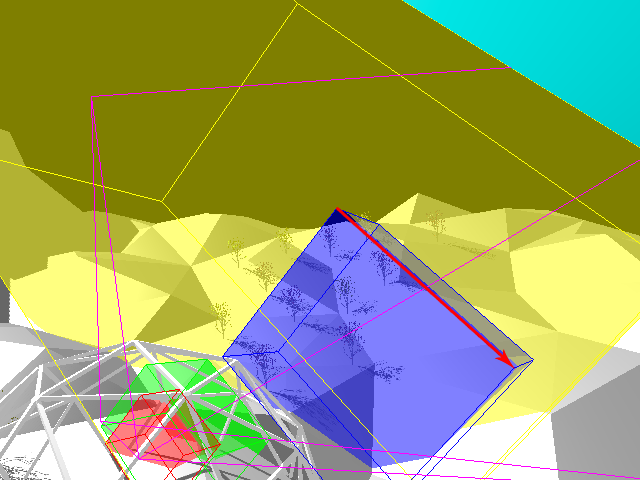
\includegraphics[width=5.5cm]{sdsm_assets/shearing/sdsm_no_shear_volumes_small_arrow.png}
		\label{ref:sdsm_light}
	}
	\subfloat [Sheared Sample Distribution Shadow Maps] {
		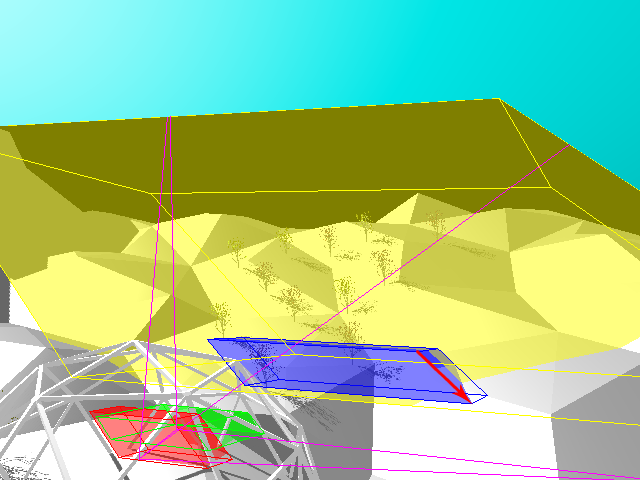
\includegraphics[width=5.5cm]{sdsm_assets/shearing/sdsm_shear_volumes_small_arrow.png}
		\label{ref:sdsm_light}
	}
	
	\caption{Visualisierung der Shadow Map Frusta. Die roten Pfeile visualisieren exemplarisch die Länge der Shadow Map Frusta entlang der Light-Space Z-Achse}
\end{figure}

Unsere Lösungsidee für dieses Problem ist eine einfache Scherung des Light-Spaces.
Die X-Achse des Camera-Spaces wird im Light-Space auf die Y-Achse abgebildet.
So haben Koordinaten, die im Camera-Space die gleiche Höhe (Y-Achse) haben, im Light-Space die gleiche Tiefe (Z-Achse).

Auch wenn wir es so schaffen in vielen Situationen die Shadow Map Frusta weiter zu verkleinern, ist durch die Scherung die Filterbarkeit der Momente \cite{msm} nicht mehr direkt gegeben.
Es ist noch relativ einfach Situationen zu provozieren, in denen die Scherung keine sinnvolle Transformation erzeugt, da dort durch einen Wert nahe $0$ geteilt wird.

\begin{equation}
	S^{-1} = \left(\begin{array}{cccc}
		1 & C_x & 0 & 0 \\
		0 & C_y & 0 & 0 \\
		0 & C_z & 1 & 0 \\
		0 & 0 & 0 & 1 \\
	\end{array}\right)
	\qquad
	S = \left(\begin{array}{cccc}
	1 & \frac{-C_x}{C_y} & 0 & 0 \\
	0 & \frac{1}{C_y} & 0 & 0 \\
	0 & \frac{-C_z}{C_y} & 1 & 0 \\
	0 & 0 & 0 & 1 \\
	\end{array}\right)
\end{equation}



% Main
\section{Volumetric Obscurance}

Volumentric Obscurance wird aus dem Screenspace berechnet. Allgemein wird für jeden Punkt der Szene, der auf
dem Bildschirm gezeichnet wird, eine gegebene Umgebung (z.B. eine Einheitskugel um diesen Punkt) betrachtet.
Für diese Umgebung wird der Anteil an Geometrie berechnet, die für den Beobachter sichtbar ist. Je mehr Geometrie
verdeckt ist, umso mehr wird der korrespondierende Pixel abgedunkelt um so den ausbleibenden Lichteinfall,
also den Schatten, zu simulieren.
Das entsprechnde mathematische Modell sieht wie folgt aus \cite{voPaper}
$$
V(P) = \int_{X} \rho (d(P,x))O(x)dx
$$
Dabei ist $X$ die Nachbarschaft um den Punkt $P$, $O$ ist die Verdeckungs-Funktion. Diese
ist 0, falls Verdeckung stattfindet, sonst 1. $\rho$ ist eine abfallende Funktion
die 1 bei P ist und mit der Distanz abfällt. Wie in \cite{voPaper} beschrieben, ist der 
sichtbare Effekt jedoch nur sehr minimal, weshalb diese Funktion als konstant angesehen 
wird \cite{voPaper}.
Im folgenden werden zwei implementierungen für Volumetric Obscurance vorgestellt:
\begin{itemize}
    \item Line Sampled Volumetric Obscurance (LSVO) (Kapitel \ref{ssec:LSVO})
    \item Area Sampled Volumetric Obscurance (ASVO) (Kapitel \ref{ssec:ASVO})
\end{itemize}

\subsection{Line Sampling} \label{ssec:LSVO}
Line Sampled Volumetric Obscurance nutzt (möglichst) zufallsverteilte Samples innerhalb auf der auf den
Screenspace projezierten Umgebung des Punktes. In der hier implementierten Version (die ebenfalls in
\cite{voPaper} beschrieben wird) wird die Einheitskugel um den Punkt P in der Szene betrachtet.
Sei nun $d$ die Tiefe des Punktes $P$. Dann ist die allgemeine Verdeckungsfunktion für eine andere Tiefe
$z$ :
$$
f(z) = \begin{cases} 1 &  \text{für } z \leq d \\ 0 & \text{für } z > d \end{cases}
$$
Für die hier vorgestellte Implementierung wird eine feste Anzahl $N$ an Samples verwendet.
Dann ergibt sich daraus für ein einzelnes LineSample:
$$
v_c = \max{(\min{(z_s, d_r)} + z_s, 0)}
$$
bzw. für eine Menge von $N$ samples:
$$
v_c = F_{N}(z_0, \dots, z_N) = \sum_i^N \frac{v_i}{2 \cdot z_{s_i}} \max{(\min{(z_{s_i}, d_{r_i})} + z_{s_i}, 0)}
$$
Dabei ist $z_i$ die Tiefe des i-ten Samples im Depth-Buffer, $d_{r_i}$ ist die Tiefe $z_i$ gemapped in die
betrachtete Umgebung des Punktes $P$, $z_{s_i} = \sqrt{1 - x_i^2 - y_i^2}$. $(x_i, y_i)$ ist die Position des
i-ten Samples auf der Einheitsscheibe (also der Querschnitt der Einheitskugel, die den Punkt P 
beinhaltet und dessen normale parallel zur Blickrichtung liegt). $v_i$ beschreibt das ``eindimensionale
Volumen'', dass die zum Sample korrespondierende Linie füllt (z.B. hat bei einer Einheitskugel genau das Sample
ein Volumen von 2, das durch $P$ geht) \newline

\begin{figure}[H]
	\centering

	\input{LineSamples.pdf_tex}
	\label{ref:lineSample}

	\caption{Line Sampling}
\end{figure}

\subsubsection{}
	\textbf{Line Sampling Pseudo Code}\\
	\begin{algorithm}[H]
		
		\Fn{LineSampling(nSamples, depth)}{
			sumSamples = 0\;
			sumVolume = 0\;
		    \For{i = 0 $\rightarrow$ nSamples - 1}{
		    	radius = $\sqrt{\text{rand()}}$\;
		    	$\alpha$ = rand()$\cdot 2\pi$\;
		    	$v_i$ = $\sqrt{1 - radius^2}$\;
		    	p = $(\cos{(\alpha)} \cdot radius,\sin{(\alpha)} \cdot radius)^T$\;
		    	sumSamples = sumSamples + $v_i$ $\cdot$ SamplePoint(p, depth)\;
		    	sumVolume = sumVolume + $v_i$\;
		    }
		    return $\frac{sumSamples}{sumVolume}$ \;
		}
		
		\Fn{SamplePoint(p, depth)}{
			\textit{hier wird ein einzelner Punkt gesampled, wie oben beschrieben} % [TODO maybe pseudocode it]
		}
		
		\Fn{rand()}{
			return \textit{zufälliger Wert im Intervall [0,1]}\;
		}
		
	\end{algorithm}
\textit{LineSampling} gibt einen Koeffizienten für die Schattierung zurück, \textit{nSamples} ist
die Anzahl der Samples, \textit{depth} die Tiefe des zum Punkt $P$ korrespondierenden Texel.

\begin{figure}[H]
	\centering
	\subfloat[1 Sample]{

		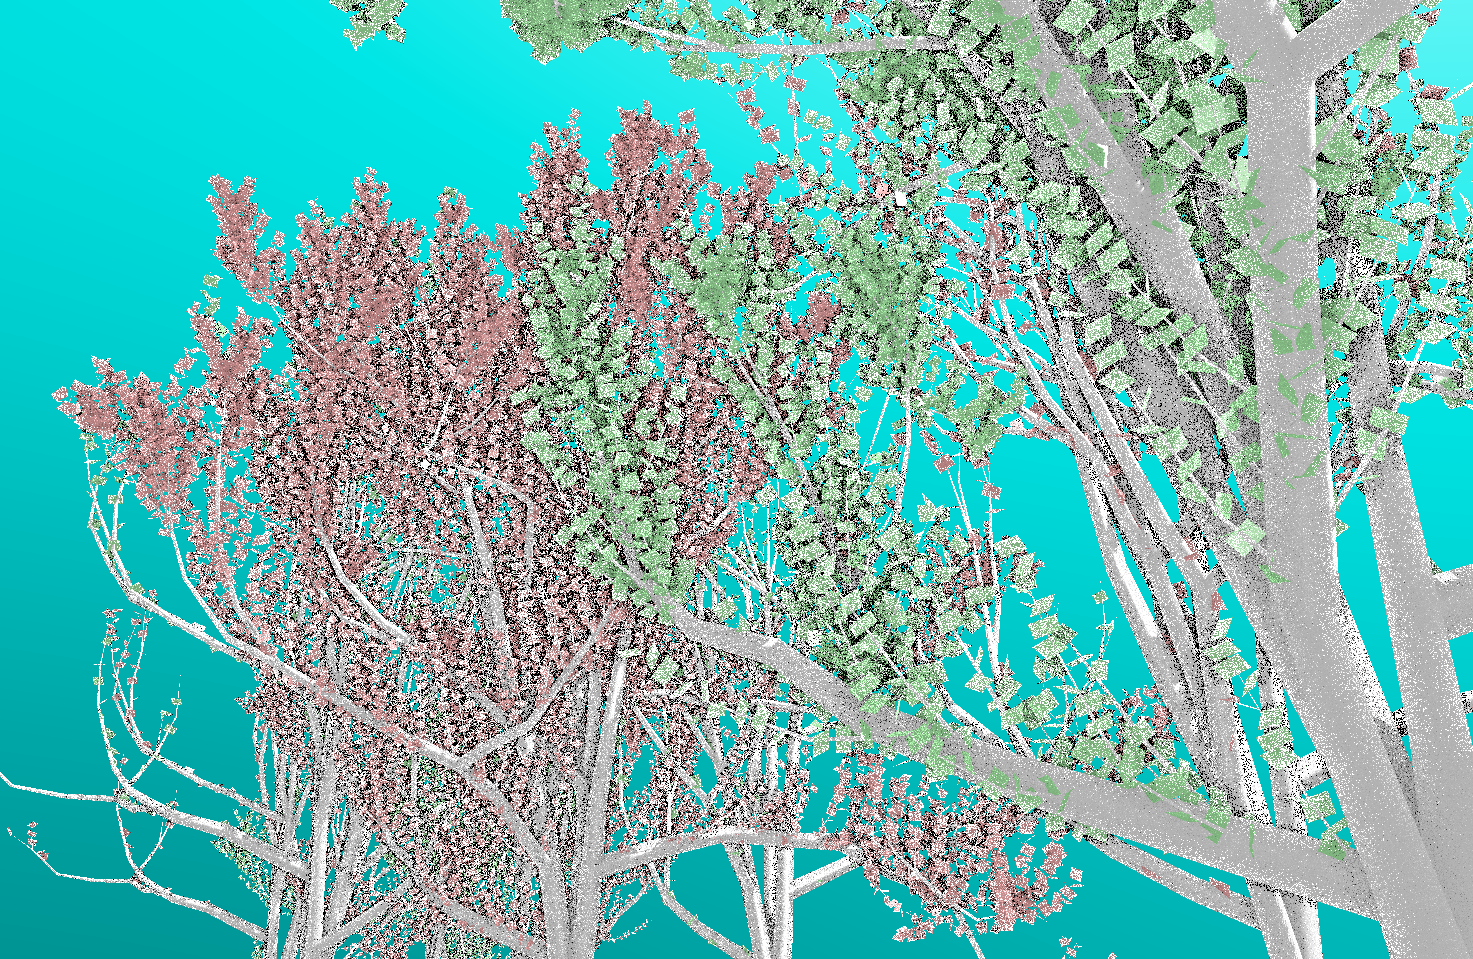
\includegraphics[width = 6cm]{vo_assets/vo_lineSample_sample0001.png}
		\label{ref:lineSample0001}
	}
    \subfloat[10 Samples]{

		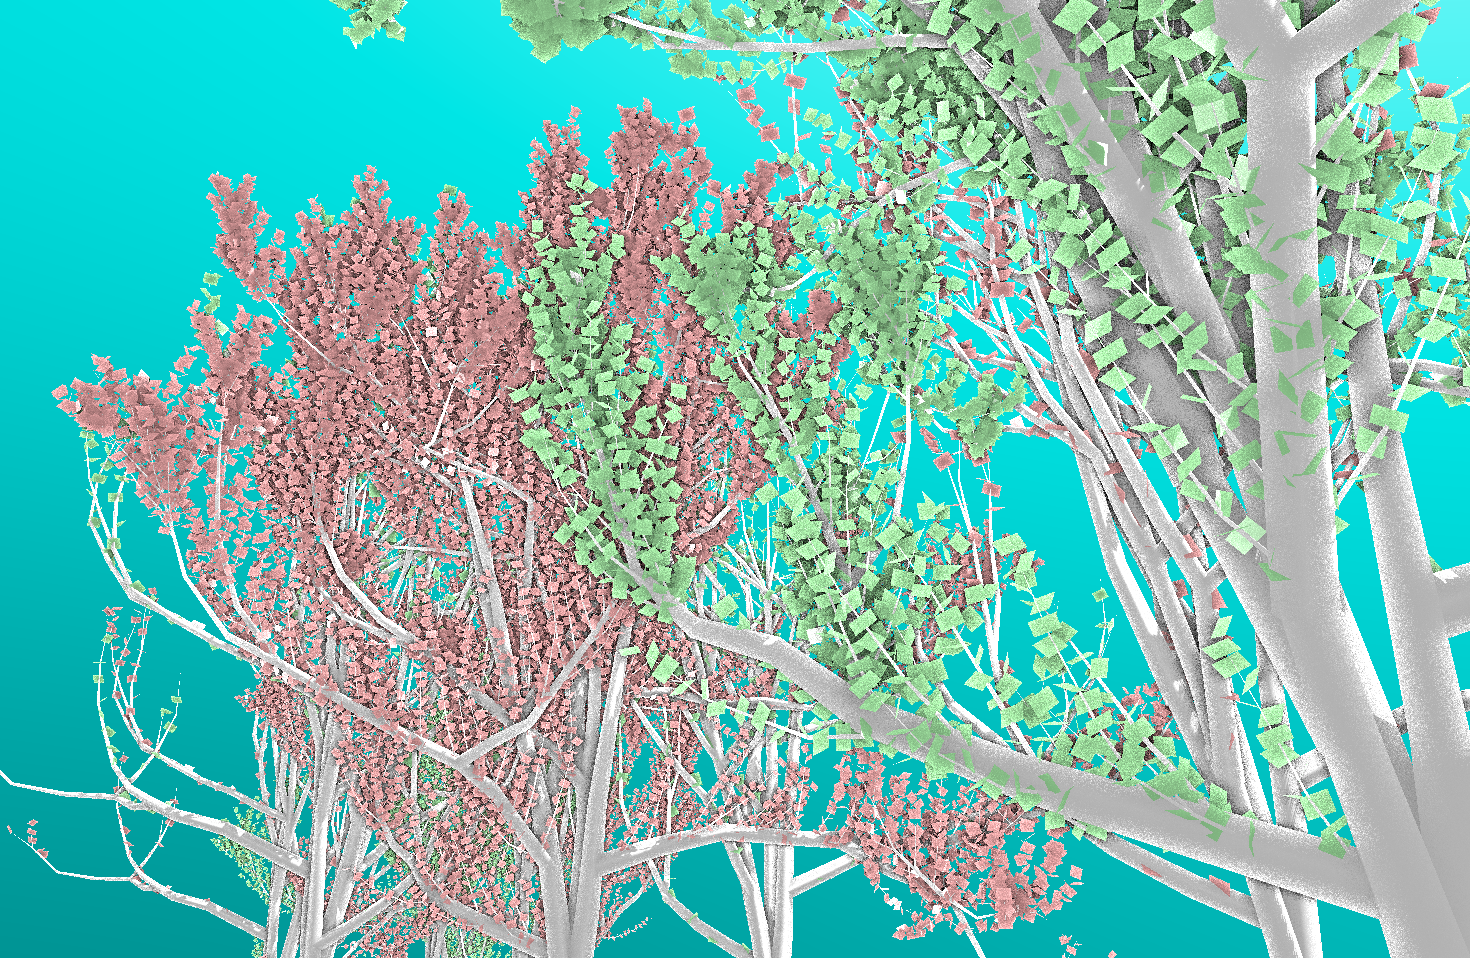
\includegraphics[width = 6cm]{vo_assets/vo_lineSample_sample0010.png}
		\label{ref:lineSample0010}
	}
	
	\subfloat[100 Samples]{
		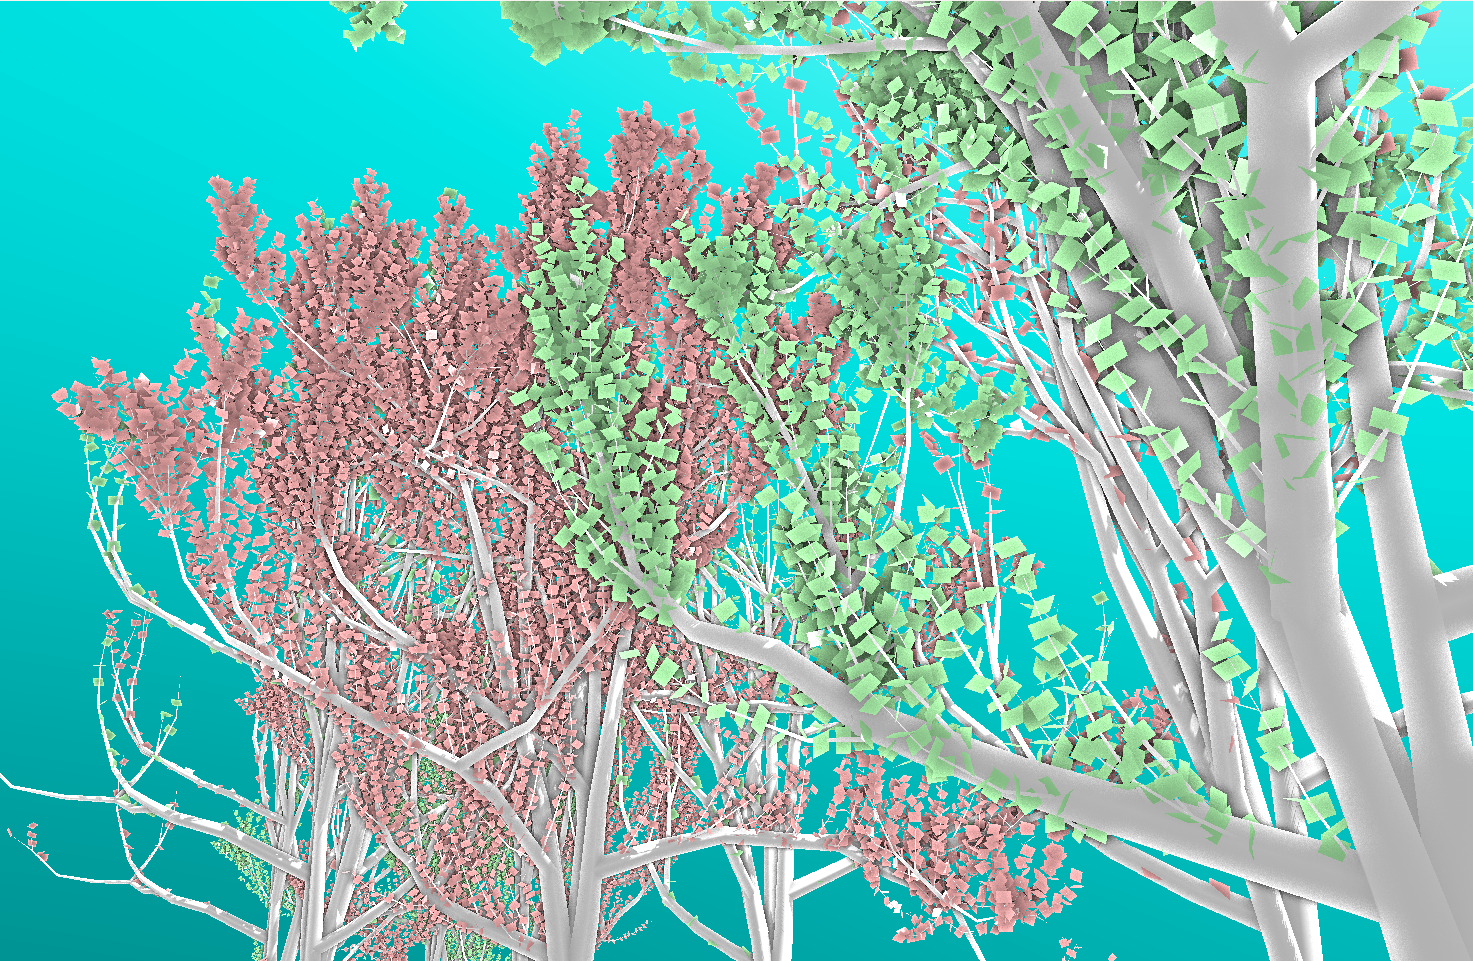
\includegraphics[width = 6cm]{vo_assets/vo_lineSample_sample0100.png}
		\label{ref:lineSample0100}
	}
	\subfloat[1000 Samples]{
		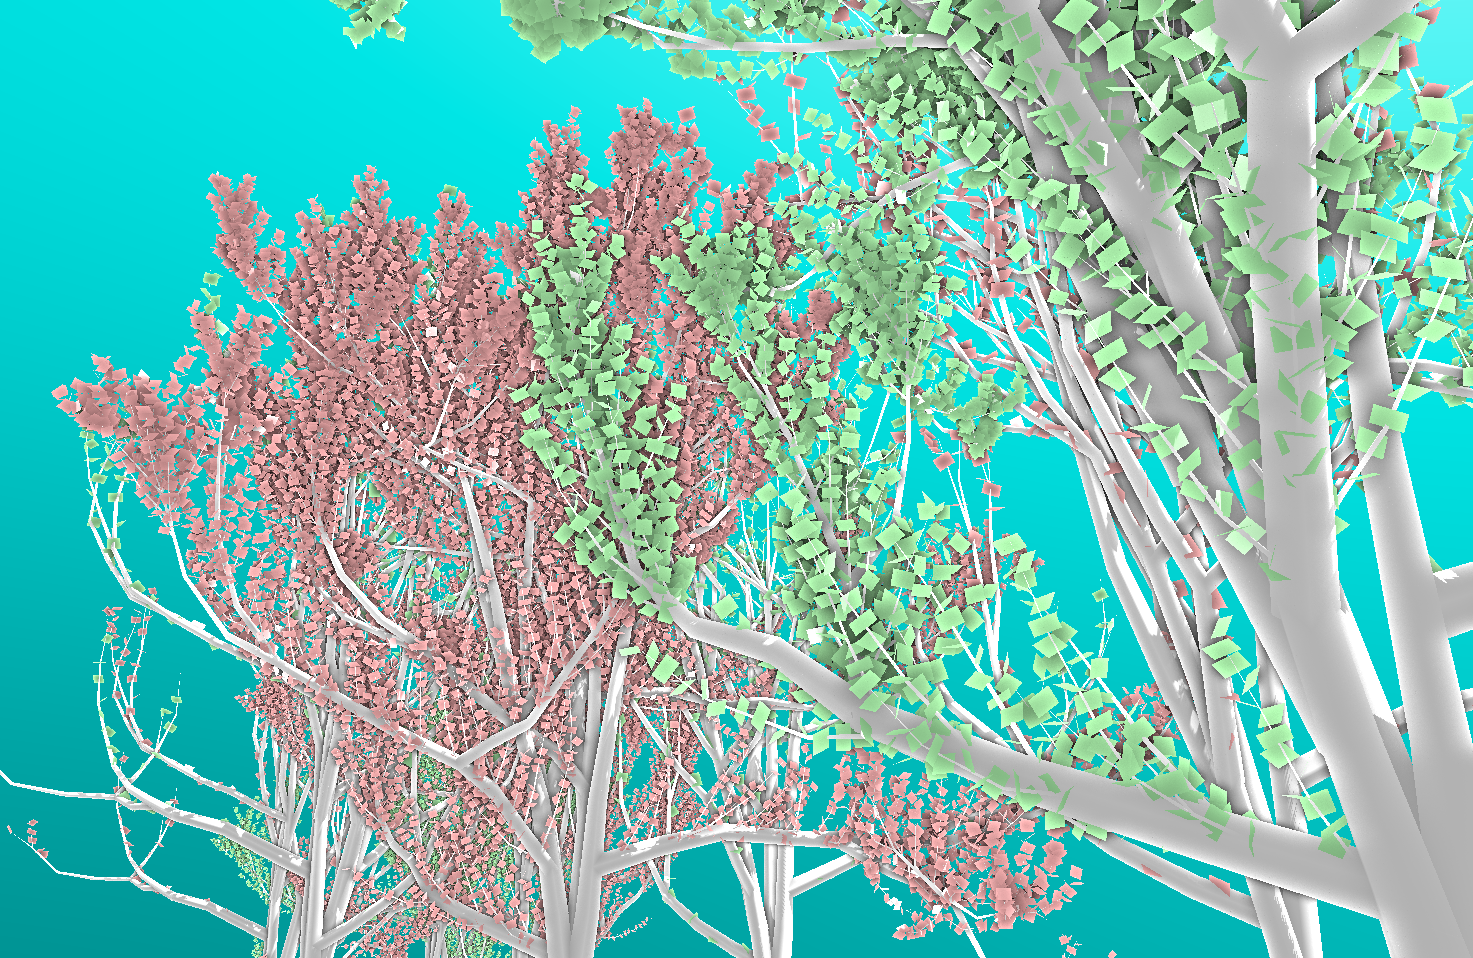
\includegraphics[width = 6cm]{vo_assets/vo_lineSample_sample1000.png}
		\label{ref:lineSample1000}
	}
	\caption{LineSampling mit verschieden vielen Samples pro Pixel}
\end{figure}

\subsection{Area Sampling} \label{ssec:ASVO}
Line Sampling Volumetric Obscurance nutzt zufallsverteilte Samples um die Verdeckung einer
Raumregion zu approximieren. Ein alternativer Ansatz ist Area Sampling. Anstatt zufallsverteilter Samples
versucht Area Sampling die Verteilung über das Mittel statistischer Größen zu ermitteln, wobei die
 grundlegende Annahme ist, dass die Tiefenwerte uniform verteilt sind. Dafür
wird der selbe Ansatz wie bei Variance Shadow Maps \cite{vsmPaper} verwendet. Beim Line Sampling
nutzten wir Samples auf dem DepthBuffer, beim Area Sampling schreiben wir stattdessen die ersten beiden
Momente $(z^1, z^2)$ für jeden Pixel im Screenspace heraus und filtern diese Größe über einen Bereich, der
Abhängig von der Tiefe ist (analog zu der von der Tiefe abhängigen, auf den Screenspace projezierten Umgebung
im Abschnitt Line Sampling). In unserer Implementierung bestimmen wir in einem Renderschritt
die Tiefe der Szene $(z)$ aus Sicht der Kamera und schreiben das Tupel $(z, z^2)$ in die ersten beiden
Farbkanälen einer Textur. Bevor wir die finale Szene rendern mipmappen wir die Textur.
In der Nachbearbeitung (Compose Schritt) der gerenderten Szene greifen wir abhängig von der Tiefe an jedem
Pixel auf die entsprechende Mipmap-Ebene zu, welche die so gefilterten Momente enthält.
Über das abgegriffene Tupel $t = (z_f, z_f^2)$ bekommen wir dann einen approximierten Mittelwert 
$\mu = t[0]$ und die gemittelte Varianz $\sigma^2 = t[1] - t[0]^2$. Dann lässt sich der Verdeckungsfaktor 
folgendermaßen abschätzen:
$$
V_c(z_0, z_1, a, b) = a\cdot(z_1^2 - z_0^2) / 2 + b \cdot (z_1 - z_0)
$$
wobei $z_0$ und $z_1$ die Start- und Endtiefe der Umgebung des betrachteten Punktes P sind und die 
Koeffizienten $a$ und $b$ definiert sind als:
$$
a = \frac{-1}{2 \cdot \sigma}; \quad b = -a \cdot (\mu + \sigma)
$$

\subsubsection{} \textbf{Pseudocode für Area Sampling:} \\
\begin{algorithm}[H]
    \Fn{AreaSampling(momentsMipmap, uv)}{
		unfilteredMoments = getMomentsFromLevel(momentsMipmap, uv, 0)\;
		depth = unfilteredMoments[0]\;
		r = getRadiusInScreenspace(depth)\;
		mipMapLevel = $\log_2 (\frac{1}{1 - r})$ \;
		moments = getMomentsFromLevel(momentsMipmap, uv, mipMapLevel)\;
		$\mu$ = moments[0]\;
		$\sigma$ = $\sqrt{ \text{moments[1]} - \mu^2}$\;
		$a$ = $\frac{-1}{2 \cdot \sigma}$\;
		$b$ = $-a \cdot (\mu + \sigma)$\;
		$z_0$ = depth - r\;
		$z_1$ = depth + r\;
		vCoeff = $V_c(z_0, z_1, a, b)$\;
		return vCoeff\;
	}
\end{algorithm}
Dabei ist \textit{getMomentsFromLevel(mipmap, uv, level)} die Funktion, die von der Mipmap \textit{mipmap}
an der Stelle \textit{uv} den Texel an gegebenem \textit{level} abgreift.
\textit{getRadiusInScreenspace(depth)} rechnet das Ausmaß der auf den Screenspace projezierten Weltumgebung
aus (in uv-Koordinaten).
Der Koeffizient \textit{vCoeff} gibt dann einen Faktor zum Einschattieren des zum Punkt $P$ korrespondierenden 
Pixels zurück. Dieser muss dann mit dem Farbwert der vorgerenderten Textur verrechnet werden (s. Abschnitt
\ref{ssec:voResult})

\subsubsection{} \textbf{Reduzierung von Artefakten} \label{sssec:SBMF}
Werden die Mipmap-Level mit Standard Mipmapping Methoden heutiger Grafik-APIs (wie z.B. glGenerateMipmaps()) erstellt, kommt es zu Artefakten im berechneten Obscurance-Term (Abb \ref{ref:SBMF_off_close}).
Um diese Artefakte zu minimieren haben wir mit dem Filtern der Momente über verschiedene Mipmap-Ebenen
experimentiert. Anstatt nur die vorgefilterten Momente über nur eine Mipmap-Ebene zu holen,
nutzen wir einen Binomialfilter (als Näherung für einen Gaußfilter) über die Mipmapebenen, mit Erwartungswert
an der Ebene, die ohne Binomialfilter gewählt werden würde. 
Sei $b_k$ das gefilterte Moment auf der k-ten Mipmapebene,
dann bekommen wir das binomail-gefilterte Moment bei einem Binomialfilter der Größe 5 mit: 

$$
b' = (\frac{1}{16}, \frac{4}{16},\frac{6}{16}, \frac{4}{16}, \frac{1}{16}) \left( \begin{array}{c} b_{(i-2)}
 \\b_{(i-1)}\\b_{i}\\b_{(i+1)}\\b_{(i+1)} \end{array} \right)
$$
In Abbildung \ref{ref:SBMF} sieht man das Ergebnis für den daraus resultierenden Obscurance Term.
\begin{figure}[H]
	\centering
	\subfloat[Area Sampling ohne LoD-Filtering]{

		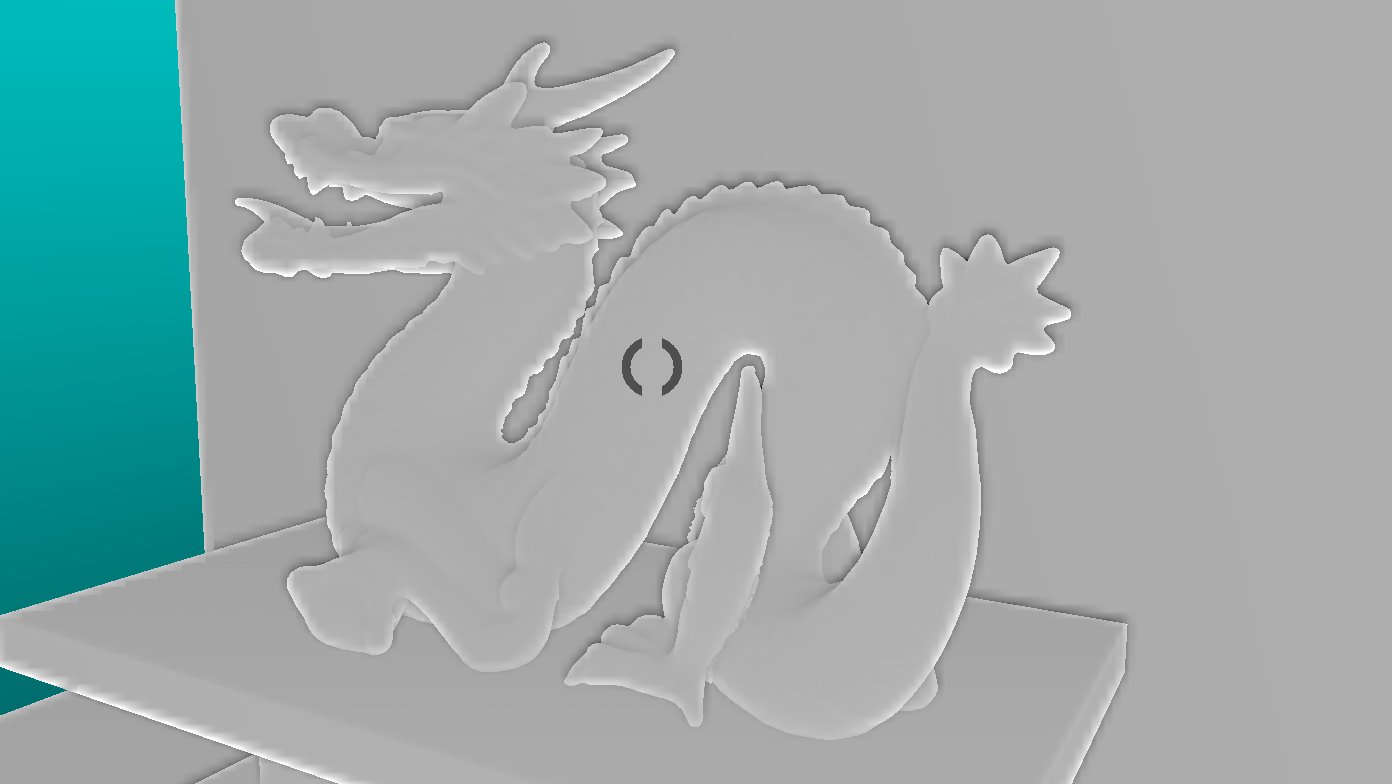
\includegraphics[width = 6cm]{vo_assets/area/shinyMMFilter_off.png}
		\label{ref:SBMF_off}
	}
    \subfloat[Area Sampling ohne LoD-Filtering]{

		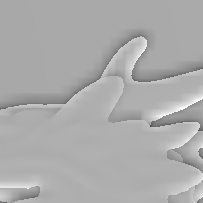
\includegraphics[width = 6cm]{vo_assets/area/zoomed/shinyMMFilter_off1.png}
		\label{ref:SBMF_off_close}
	}
	
	\subfloat[Area Sampling mit LoD-Filtering]{

		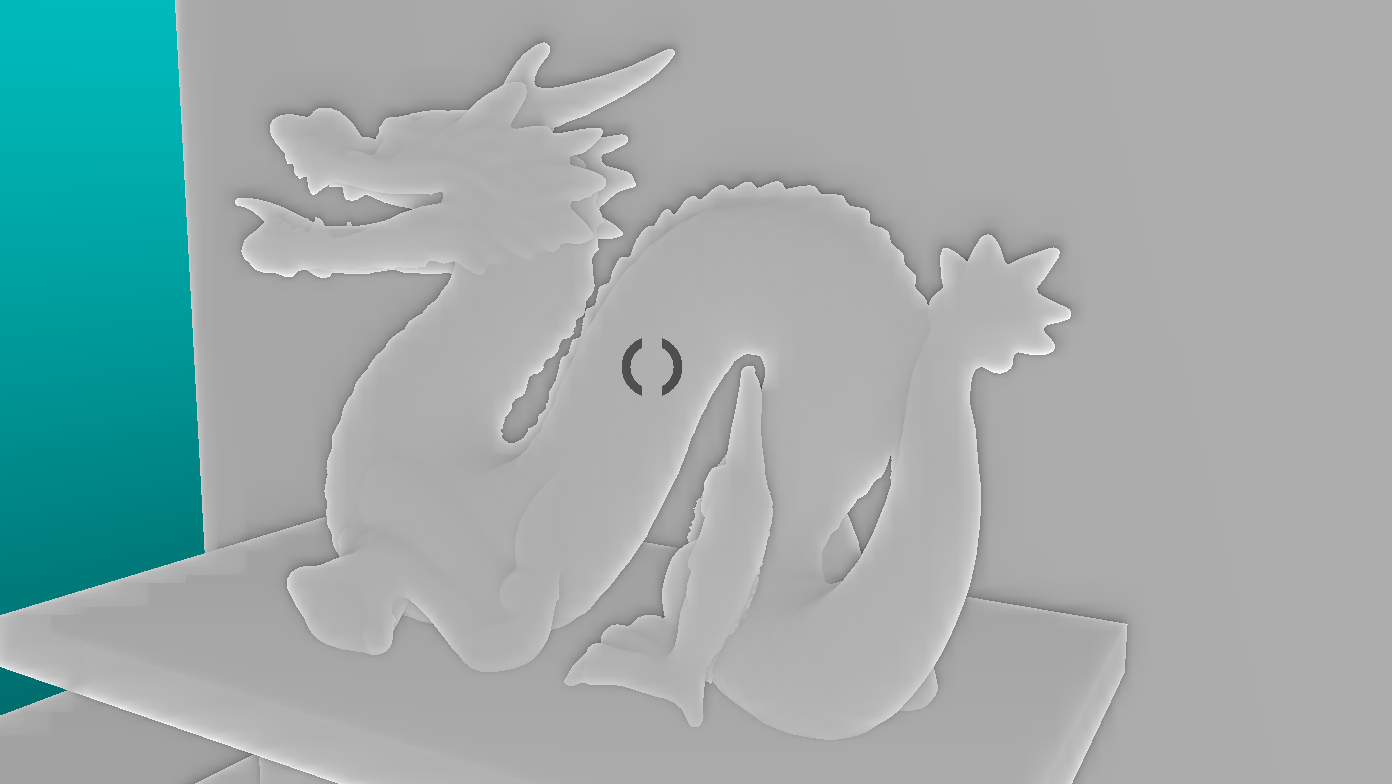
\includegraphics[width = 6cm]{vo_assets/area/shinyMMFilter_on.png}
		\label{ref:SBMF_on}
	}
    \subfloat[Area Sampling mit LoD-Filtering]{

		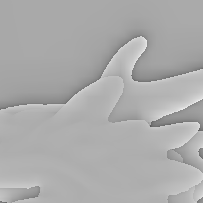
\includegraphics[width = 6cm]{vo_assets/area/zoomed/shinyMMFilter_on1.png}
		\label{ref:SBMF_on_close}
	}
	\caption{Ergebnisse mit binomialem LevelofDetail (LoD) Filtering}
	\label{ref:SBMF}
\end{figure}

% Main
\section{Moment Shadow Mapping}
%Neuer Teil:
VSM bietet uns bereits einen Ansatz für gefilterte Shadow Maps, besitzt aber auch noch ein paar Nachteile wie das angesprochene Light-Leaking. Wir möchten das Verfahren erweitern und 4 Momente nutzbar machen, um dunklere Schattenintensitäten zu erreichen und ein noch hochwertigeres Bild zu erhalten.\\
Hierfür Nutzen wir das Hamburger Moment Shadow Mapping (im weiteren Verlauf MSM).
Unser Ziel ist es eine Shadow Map mit 4 Kanälen zu nutzen, welche jeweils 16bit haben. Dadurch möchten wir eine gute Heuristik für gefilterte Hard Shadows, mit geringen Kosten erreichen. Wie bereits angesprochen, gibt uns VSM bereits eine untere Schranke, sodass die Tiefenfunktion bereits oberhalb dieser liegen.\\
Desweiteren ist eine Minimierung der Wahrscheinlichkeit an einer bestimmten Tiefe wünschenswert, was im allgemeinen als General Moment Problem betitelt wird.\\
Dies wird durch eine Funktion mit verallgemeinerten Momenten gelöst. Die verallgemeinerten Momente werden durch eine zufällige Vektorvariable beschrieben. Diese definiert was in der Shadow Map gespeichert wird. Beispielsweise ist dies für VSM $b(z) = (z,z^2)$ oder für das angestrebe MSM $b(z) = (z,z^2,z^3,z^4)$. Die Werte der Momente dienen als Eingabe.\\
Zusammengefasst möchten wir alsoe eine Auswahl eines Kandidaten aus der ShadowMap Heristik treffen. Desweiteren streben wir eine Verbesserung des Ergebnisses durch eine 4 Kanal Shadow Map an. Die beste Möglichkeit für Echtzeitrendering bietet hier das Hamburger Moment Shadow Mapping. Der vollständigkeithalber, sei gesagt, das etwa Trigonometrisches MSM optima gewesen wäre. Allerdings ist es zu kompliziert und unstabil, wenn auch besser gegen Light Leaking anwendbar. Dennoch ist es wünschenswert, ein Verfahren zu nutzen das auch für Echtzeitverfahren nutzbar ist.\cite{msm}\\
% MSM
\subsection{Algorithmus: Moment Shadow Mapping}
%untere Schranke
Für jede Tiefe, benötigen wir eine Funktion mit Momenten, welche uns diese minimale Wahrscheinlichkeit an dieser Tiefe liefert. Diese wird jedesmal durch eine stückweise Konstante Funktion mit 3 Anstiegspunkten erreicht. Einer dieser Anstiegspunkte ist jener, den wir minimeren möchten. Dies folgt aus dem Markov-Krein Theorem.\cite{msm}\\
Desweiteren müssn die bediden anderen Anstiegspunkte berechnet werden. Dies kann durch folgende Gleichung gelöst werden:
$$b_j = E_z(z^j)$$
$$\begin{pmatrix} 
1\\
z_{2/3}\\
z^2_{2/3}\\
\end{pmatrix}^T \cdot 
\begin{pmatrix}
1 & b_1 & b_2\\
b_1 & b_2 & b_3\\
b_2 & b_3 & b_4\\
\end{pmatrix}^{-1} \cdot
\begin{pmatrix}
1\\
z_f\\
z^2_f\\
\end{pmatrix} = 0
$$
Der Algorithmus sieht dann wie folgt aus:\\
\\
\textbf{Input}: Tiefe $z_f \in \mathbb{R}$, Momente $b_j = \mathbb{E}_z(z^j)$ für $j \in \{1,2,3,4\}$.\\
\textbf{Output}: Approximierte Schattenintensität.\\
\begin{enumerate}
\item $$\text{Löse}
\begin{pmatrix}
1 & b_1 & b_2\\
b_1 & b_2 & b_3\\
b_2 & b_3 & b_4\\
\end{pmatrix} \cdot
\begin{pmatrix} 
c_1\\
c_2\\
c_3\\
\end{pmatrix}  =
\begin{pmatrix}
1\\
z_f\\
z^2_f\\
\end{pmatrix} = 0
$$
\item $$\text{Löse} \;
c_3 \cdot z^2 + c_2 \cdot z + c_1 = 0\; \text{für} \; z_2,z_3 \in \mathbb{R} 
$$
\item $$ \text{Löse}
\begin{pmatrix}
1 & 1 & 1\\
z_f & z_2 & z_3\\
z^2_f & z^2_2 & z^2_3\\
\end{pmatrix} \cdot
\begin{pmatrix} 
w_1\\
w_2\\
w_3\\
\end{pmatrix}  =
\begin{pmatrix}
1\\
b_1\\
b_2\\
\end{pmatrix}
$$
\item 
$$
\text{Return:} \;
\sum_{i=1,z_i<z_f}^{3} w_{i}
$$
\end{enumerate}

Der Algorithmus beginnt mit dem berechnen der beiden unbekannten Anstiegspunkten (1).
Dies sind die Wurzeln aus der quadratischen Gleichung (2). Die Koeffizienten dieser Gleichung sind die Ergebnisse eines linearen 3x3 Gleichungssystems (3).
Nach dem berechnen dieser 3 Anstiegspunkte, muss ein weiteres lineares 3x3 Gleichungssystem (3) gelöst werden, um die Gewichte $w$ zu erhalten, welchte die korrekten Momente produzieren. Schließlich nutzen wir die Gewichte und die Anstiegspunkte um die Wahrscheinlichkeit zu berechnen (4).\cite{msm}
\subsection{Algorithmus: Moment Based Volumetric Obscurance}
Moment Based Volumetric Obscurance funktioniert grundlegend wie das bereits beschriebene Volumetric Obscurance mit Area Sampling. Allerdings nutzen wir für als Filter Region den Tiefen Buffer, welcher uns eine wohldefinierte, aber unbekannte Z Funktion, mit linearen Tiefenwerten liefert. Hier machen wir uns die Moment Technik zunutze, da wir diese Funktion durch 4 Momente beschreiben können, welche uns zunächst wenige Informationen liefern. Ähnlich wie beim Moment Shadow Mapping können wir dies also folgendermaßen beschreiben:
$$ b := E_z(b) \in \mathbb{R}^m $$
Wir versuchen also einen Term für die Volumetric Obscurance, auf Basis der Tiefeninformationen zu approximieren. Ausserdem möchten wir den Obscuranceterm in einem Tiefeninterval von $z_a$ $\in$ $\mathbb{R}$ bis $z_b$ $\in$ $\mathbb{R}$ berechnen.
Hierraus ergibt sich folgender Term durch $\mathbb{E}_z(f)$: 
$$ f(z)
\begin{cases}
\phantom{} 1 & \text{falls } z < z_a\\ 
\frac{z-z_a}{z_b-z_a} & \text{falls } z_a \leq z \leq z_b\\
0 & \text{falls } z_b < z
\end{cases}
$$
Unsere Annahme hierfür basiert darauf, dass es nicht mehr als 3 unterschiedliche Tiefenwerte in der gerade betrachteten Region gibt, gegeben durch $n:=\frac{m}{2}+1$ mit $m=4$ (Momenten). Dies sind also jene Tiefenwerte die wir durch die Z Distribution betrachten. Wir wissen, dass eine der Tiefenwerte durch $z_f$ beschrieben wird, wenn dieser ist das einzig explizit gegebene sample aus der Filter-Region. Durch dieses Wissen können wir eine Funktion $S$ aufstellen, mit unterstützung von $z_1=z_f$ und weiteren Stützpunkten $z_2,...,z_n \in \mathbb{R}$  und den korrekten Momenten $\mathbb{E}_s(b)=b$. Diese können wir schreiben als:
$$ 
S = \sum_{i=1}^{n} w_i \cdot \delta_{z_i} 
$$
Hier lässt sich bereits der Bezug zum Moment Shadow Mapping herstellen. Desweiteren wird $\delta_{z_i}$ als Diraksche Delta Funktion verstandten mit unterstützung bei $z_i$ und $w_1,...,w_n \in [0,1]$.
Dies kann durch das Moment Shadow Mapping bzw. dessen Techniken robust und effizient berechnet werden, indem wir das Verfahren noch etwas modifizieren:
$$ 
\mathbb{E}_s(f) = \sum_{i=1}^{n} w_i \cdot f_{z_i} 
$$
Durch Anpassung des MSM Algorithmus, können wir also einen Term für die Volumetric Obscurance berechnen, welches in der Implementierung wenig Anpassung benötigte.
Diese Herangehensweise stammen aus den Notizen von Christoph Peters\cite{mbvo}.

% MSM
\subsection{Implementierung}
Für die Implementierung des MSM Algorithmuses hatten wir HLSL Code gegeben \cite{msm}.
Diesen haben wir für GLSL umgeschrieben, was nur wenig Anpassungen benötigte und leicht umseztbar war.\\
Für das rendern der Shadow Map benötigten wir eine 4 Kanal Textur. Diese speichert die Momente $z,z^2,z^3,z^4$. Die Momente werden bei uns in einem eigenen Shader erstellt. Da diese nicht mit Double Precision Werten gespeichert werden können, denn dies würde zu unakzeptabler Speichernutzun führen, müssen diese noch komprimiert werden. Damit der Informationsverlust bei der Quantifizierung gemindert wird, nutzen wir einen Biased Moment Vektor. Ausserdem sind 16 bit pro gespeichertem Moment hierfür wünschenswert, was uns zu einer weiteren Quantifizierung führt. Beides hatten wir bereits im Algorithmus gegeben und konnten dies einfach übernehmen um das Hamburger Moment Shadow Mapping umzsetzen.\\
Die gesampelten Momente werden im Fragment Shader eingelesen und weiter verarbeitet, wie im Algorithmus-Teil beschrieben. Nun hatten wir auch die Möglichkeit Filtern und Anti-Aliasing anzuwenden.˜˜
Wir haben wir uns für Gauss Filtern, mit einem 9x9 Kernel, sowie Multi Sample Anti-Aliasing (MSAA) entschieden. Beides wird durch die Momente ermöglicht, da diese nun gefiltert und anti-aliased werden können. MSAA sorgt wie Super Sampling dafür, dass Kanten weicher erscheinen. MSAA kann auf der Grafikhardware berechnet werden und ermöglicht es, bei schrägen Linien, jeden benachbarten Pixel mit seinen Nachbarpixeln zu vergleichen. Die Farben werden so angepasst, das eine weichere Kante entsteht. Dadurch erreichen wir, das unsere Schatten nicht mehr so stark von der Treppchenbildung des Aliasing betroffen sind. \\Der Gauss Filter hat einen ähnlichen Effekt. Allerdings wirkt das Bild verwaschener und ähnelt eher Softshadows. Wir haben beides so implementiert, das es auch zusammen genutzt werden kann. Ausserdem kann MSAA von 1-fach bis 16-fach genutzt werden, was allerdings viel Leistung benötigt.\\
Letzendlich können wir die Schattenintensität berechnen.
Die Funktionen rufen wir in der simpleShadowTerm() Funktion auf und geben diese letzendlich als Wert für die Textur zurück.
\begin{figure}[H]
	\centering
	\subfloat[Tiefe]{

		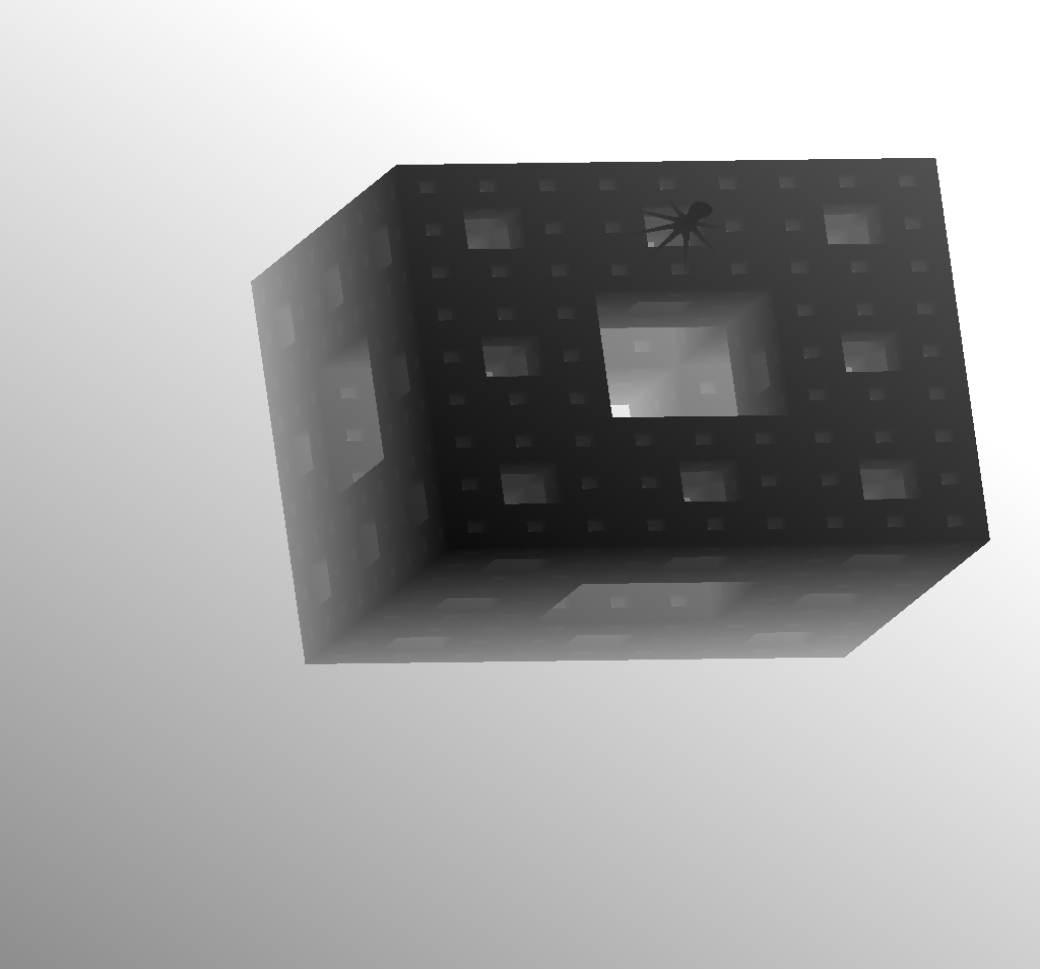
\includegraphics[width = 6cm]{msm_assets/depthbuffer/menga_depth.png}
		\label{ref:momentz}
	}
    \subfloat[aus Tiefe generierte Momente]{

		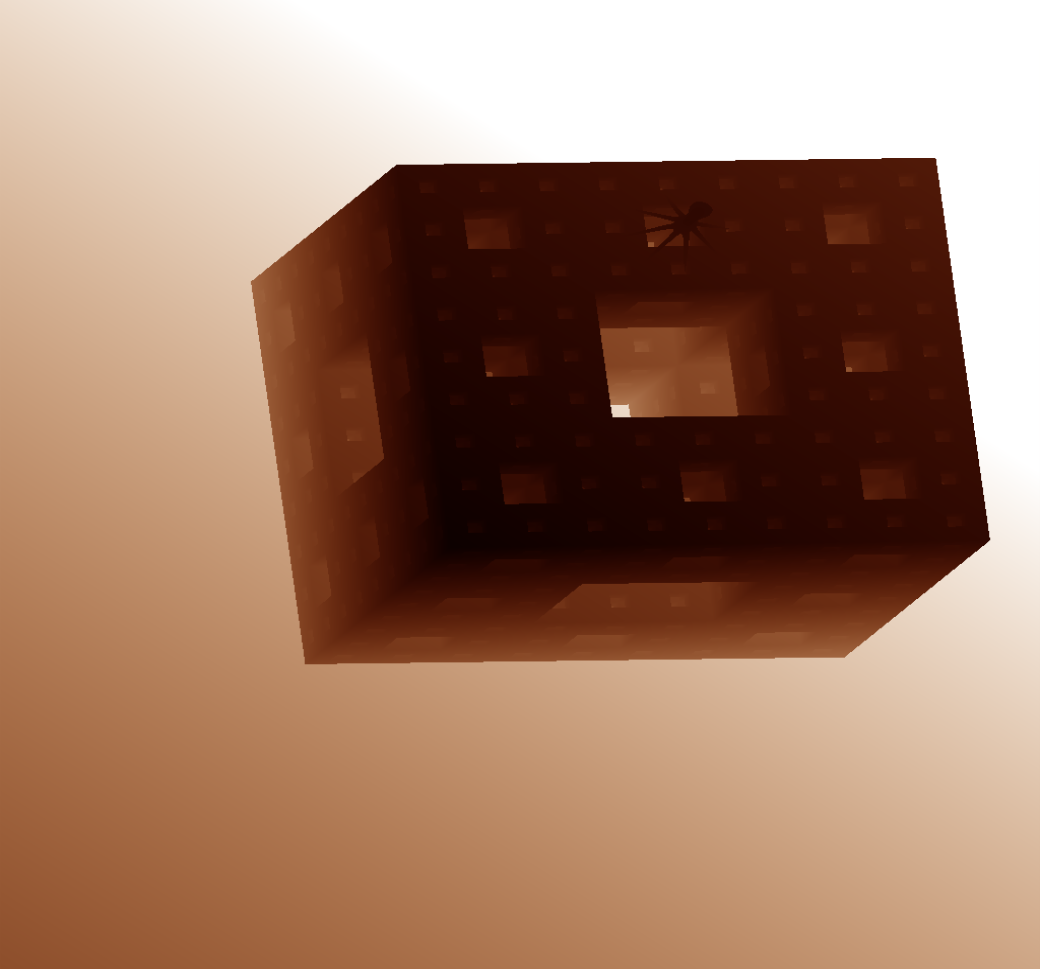
\includegraphics[width = 6cm]{msm_assets/depthbuffer/menga_moments.png}
		\label{ref:momentnew}
	}
	
	\subfloat[ungefilterte Momente]{
		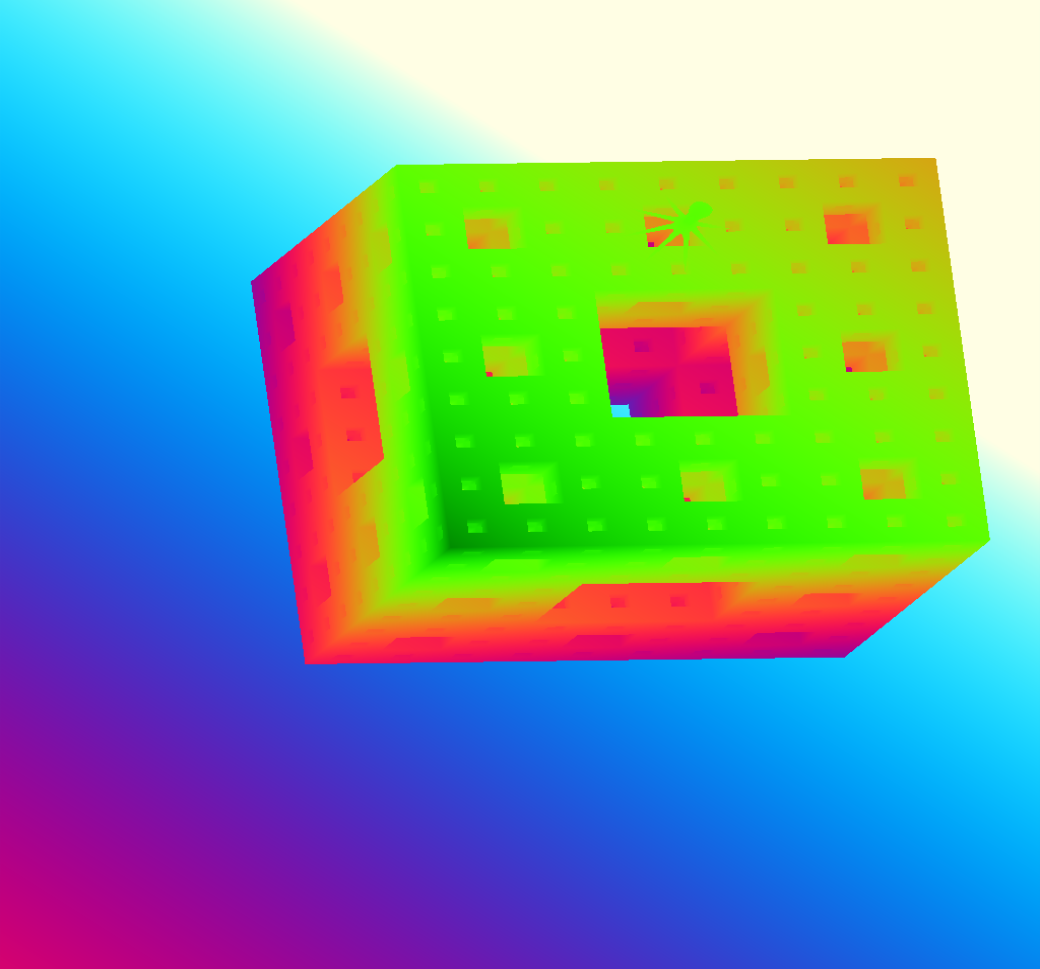
\includegraphics[width = 6cm]{msm_assets/depthbuffer/menga_transformed.png}
		\label{ref:momentcalc}
	}
	\subfloat[Gauss Filter und Momente]{
		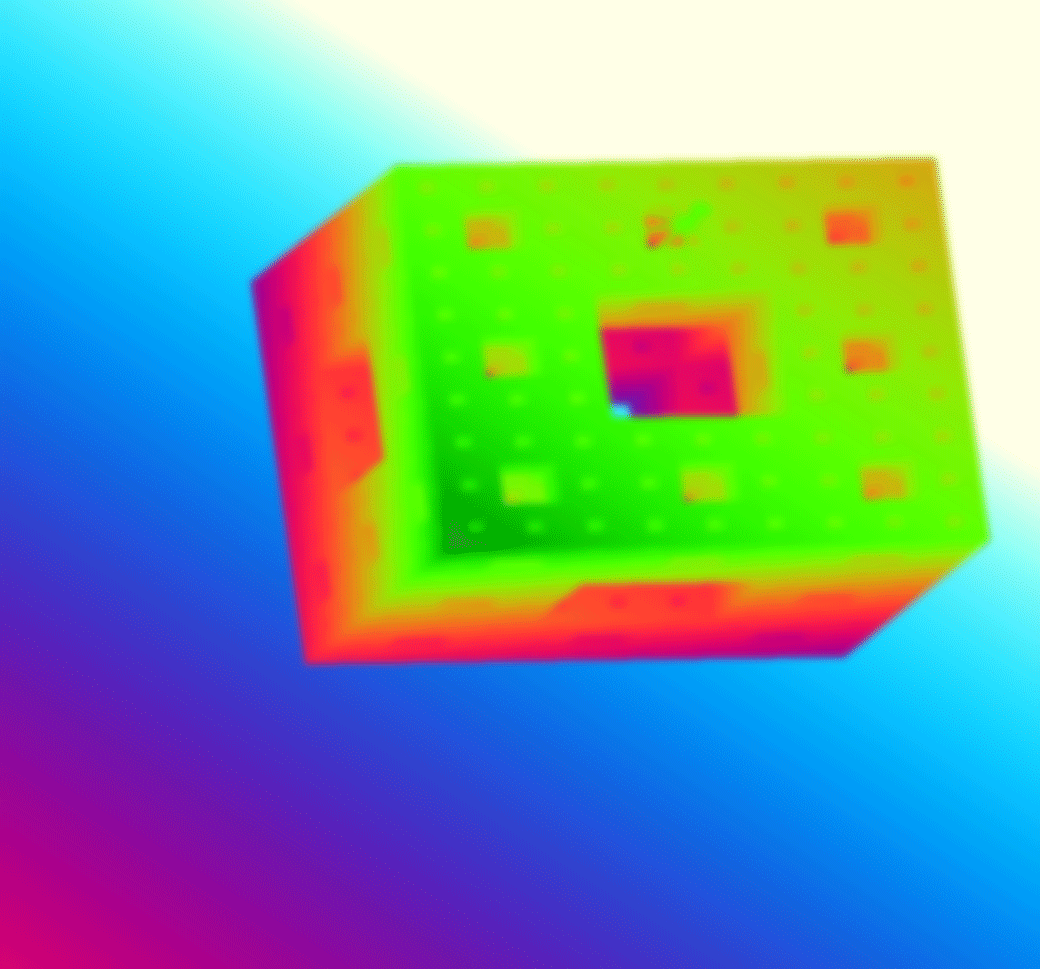
\includegraphics[width = 6cm]{msm_assets/depthbuffer/menga_transformed_gauss.png}
		\label{ref:momentgauss}
	}
	\caption{Die Bilder zeigen den Tiefenwert aus Depth Buffer, generierte Momente aus create\_moment.glsl Shader und schließlich mit Gauss gefilterte Momente zum Verlgleich}
\end{figure}
\subsection{Implementierung: Moment Based Volumetric Obscurance}



Für das Moment Based Volumetric Obscurance benutzen wir die gleiche Herangehensweise.
Aus dem Algorithmus für das MSM haben wir die Gewichte $w_i$ ausgelesen und konnten hiermit den Term für die Volumetric Obscurance berechnen, wie im Abschnitt Algorithmus beschrieben. Hierfür waren nur wenig Anpassungen am gegeben HLSL Code nötig um diese in die beschrieben Volumetric Obscurance einzusetzen. Das weitere Verfahren entspricht dem aus dem Abschnitt Area Sampling, welches nur durch die Momente angepasst wurde. \\
Desweiteren haben wir 32-bit für die Momente genutzt. Deswegen war eine Quantifizierung nicht nötig.\\
Allerdings hat es sich herausgestellt, dass die OpenGL beim Mip-Mappen der 4 Momente zu Artefakten führt. Dies entspricht dem samplen im Fragment Shader aus der Implementierung des Moment Shadow Mapping. Problematisch ist hier der Umgang mit dem Alpha Kanal, da dieser den 4. Moment nicht korrekt darstellt und so keinen  korrekten Wert für die Vomuletric Obscurance liefert. Deswegen mussten wir zwei 2-Kanal Texturen nutzen um die 4 Momenten auf diese aufzuteilen. Danach funktionierte das Mip-Mapping.



\section{Fazit}


% Fazit
\subsection{Sample Distribution Shadow Maps}
SDSMs sind sehr robust und benötigen keine möglicherweise von Hand zu optimierenden Parameter um gute Ergebnisse zu erzielen.
PSSMs können oft ähnlich gute Ergebnisse liefern wenn sie optimal eingestellt sind.
Allerdings gilt dies meist nur für eine bestimmte Sicht auf die Szene.
Befindet sich mehr oder weniger Geometrie in unmittelbarer nähe zur Kamera, so liefert PSSM keine guten Ergebnisse mehr.
SDSM passt ihre Z-Partitionen adaptiv an die veränderte Sichtbarkeit an.
Dies ist möglich, da SDSMs die tatsächliche Near Plane kennen, wo PSSMs nur eine untere Schranke hierfür kennen, die sich aus der Kamera Projektion ergibt.

% Verbesserung der MSM durch SDSM
% TODO erstmal nur skizziert!
SDSMs optimieren nicht nur die Ausnutzung der Shadow Map Auflösung, sondern auch die Ausnutzung der zur Verfügung stehenden Genauigkeit in der Shadow Map, da die Shadow Map Frusta in allen drei Dimensionen eng um die sichtbare Geometrie gelegt wird.
Dies kommt dem Moment Shadow Mapping zu gute, da so feinere Abstufungen in den Momenten erlaubt werden.

Sheared Sample Distribution Shadow Maps sind eine vielversprechende Methode um die Quantifizierung der Shadow Map in flachen Szenen besser auszunutzen.
Es handelt sich jedoch bisher nur um eine Idee.
Wie genau die Scherung bestimmt werden kann ohne in die Nähe von Singulatitäten zu gelangen muss noch evaluiert werden.


% Fazit
\subsection{Volumetric Obscurance} \label{ssec:voResult}
Wie erwartet sehen SSAO (Abb \ref{ref:crytekSSAO}) und Line Sampled Volumetric Obscurance 
(Abb. \ref{ref:LSVO010}, Abb. \ref{ref:LSVO100}) sich sehr ähnlich. 
Area Sampled Volumetric Obscurance (Abb. \ref{ref:ASVO})
lieferte in unserer Implementierung ebenfalls gute Resultate und bietet so eine Alternative 
zum relativ teuren Line Sampled Volumetric Obscurance. 

\begin{figure}[H]
	\centering
	\subfloat[SSAO by Crytek \cite{cry2Paper}]
	{

		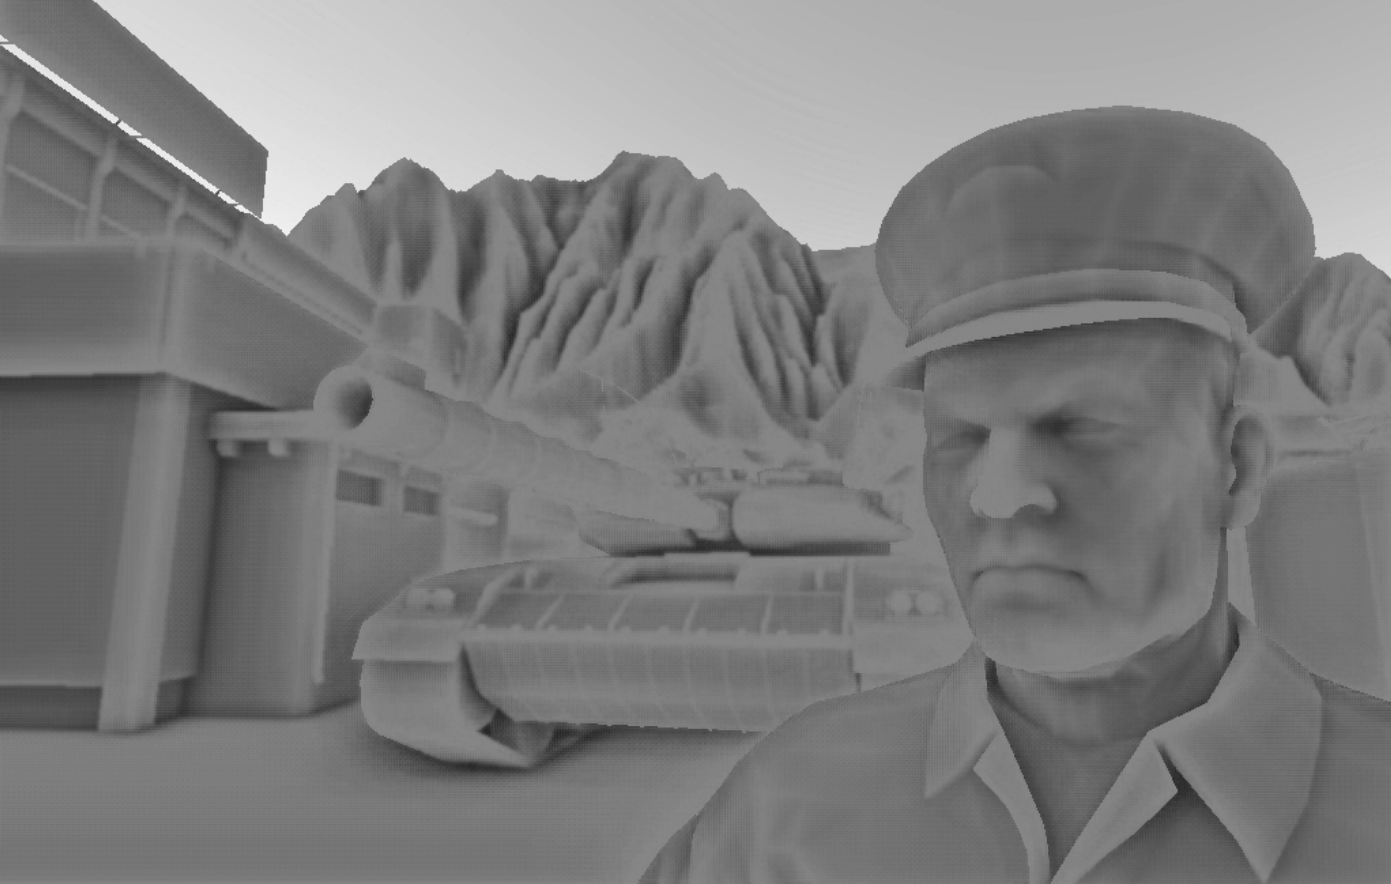
\includegraphics[width = 6cm]{vo_assets/crytekSSAO.png}
		\label{ref:crytekSSAO}
	}
	\subfloat[Line Sampled Obscurance Term mit 10 samples]
	{

		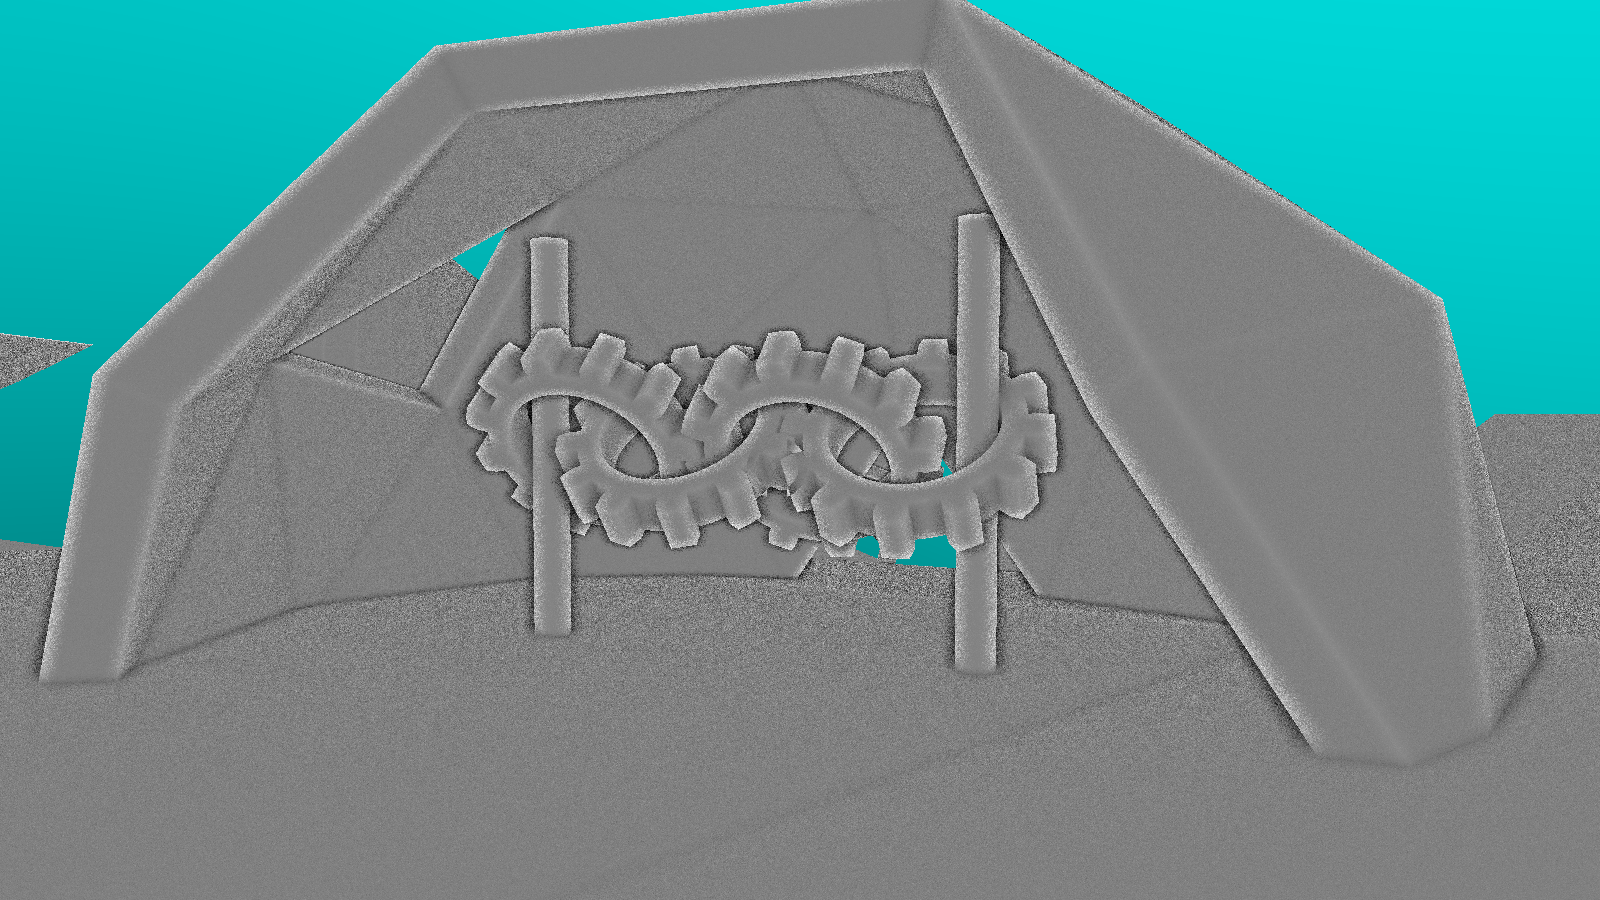
\includegraphics[width = 6cm]{vo_assets/presentaton_graphics/dome/LSVO_only_10.png}
		\label{ref:LSVO010}
	}
	
	\subfloat[Line Sampled Obscurance Term mit 100 samples]
	{

		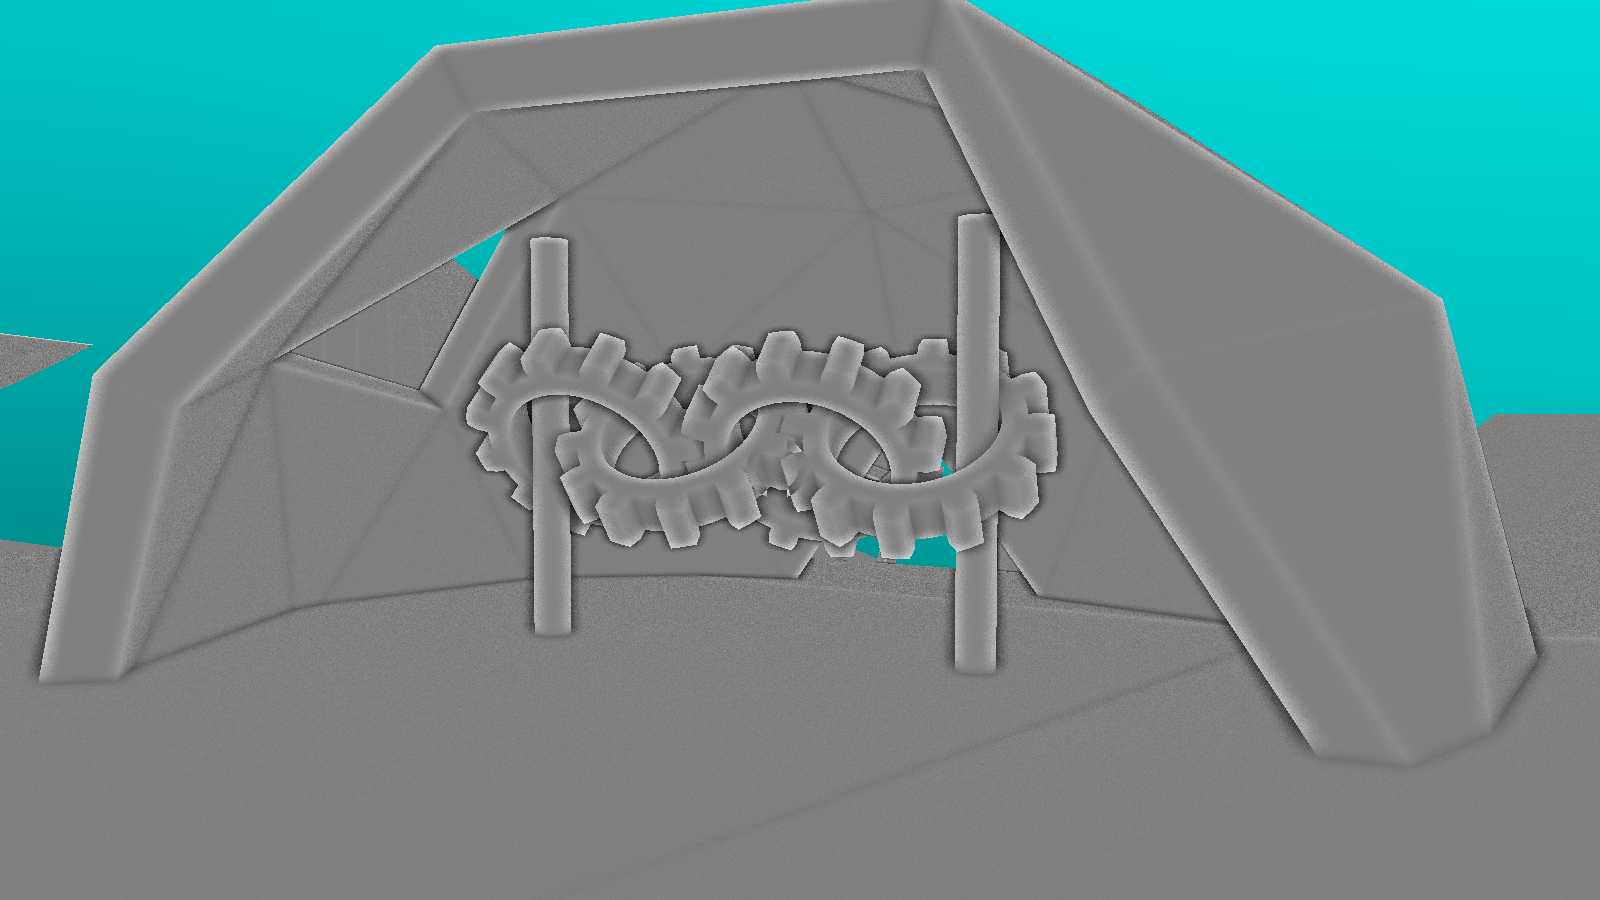
\includegraphics[width = 6cm]{vo_assets/presentaton_graphics/dome/LSVO_only_100.png}
		\label{ref:LSVO100}
	}
	\subfloat[Area Sampled Obscurance Term]
	{

		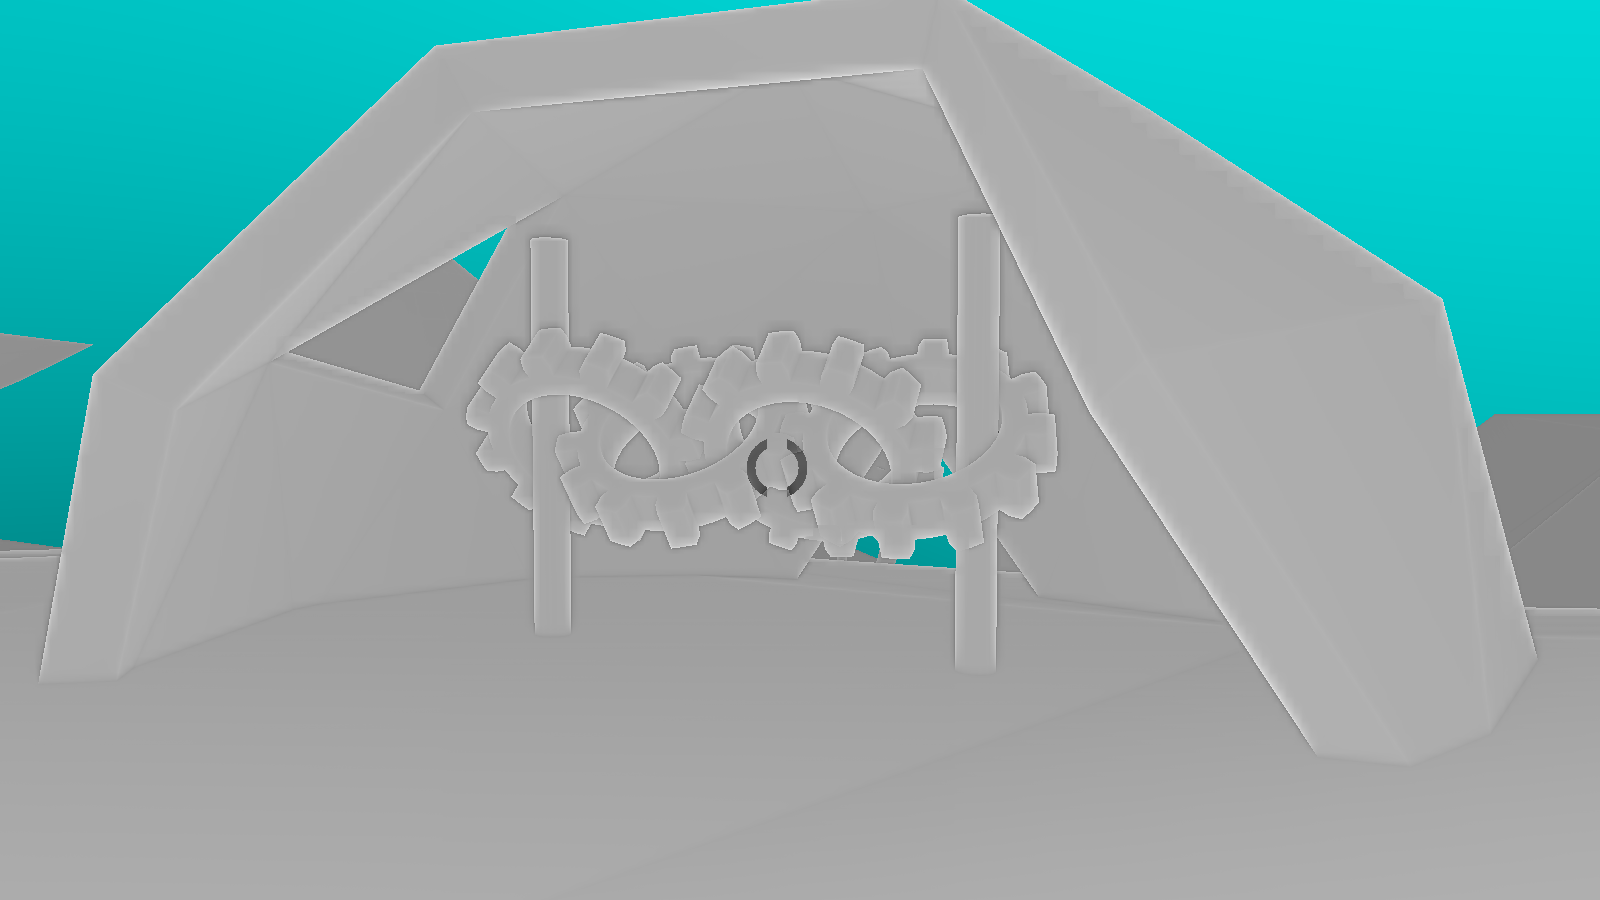
\includegraphics[width = 6cm]{vo_assets/presentaton_graphics/dome/ASVO_only.png}
		\label{ref:ASVO}
	}
	\caption{Resultate von Umgebungsverdeckungstechniken}
\end{figure}
In Abbildung \ref{ref:finalVO} sieht man gut im Vergleich, wie Volumetric Obscurance Objekte sichtbar macht,
die bei einem Rendering nur mit Shadowmapping und ohne Global Illumination Techniken nicht sichtbar wären.
\begin{figure}[H]
	\centering
	\subfloat[Rendering ohne VO: Zahnräder sind nicht sichtbar]
	{

		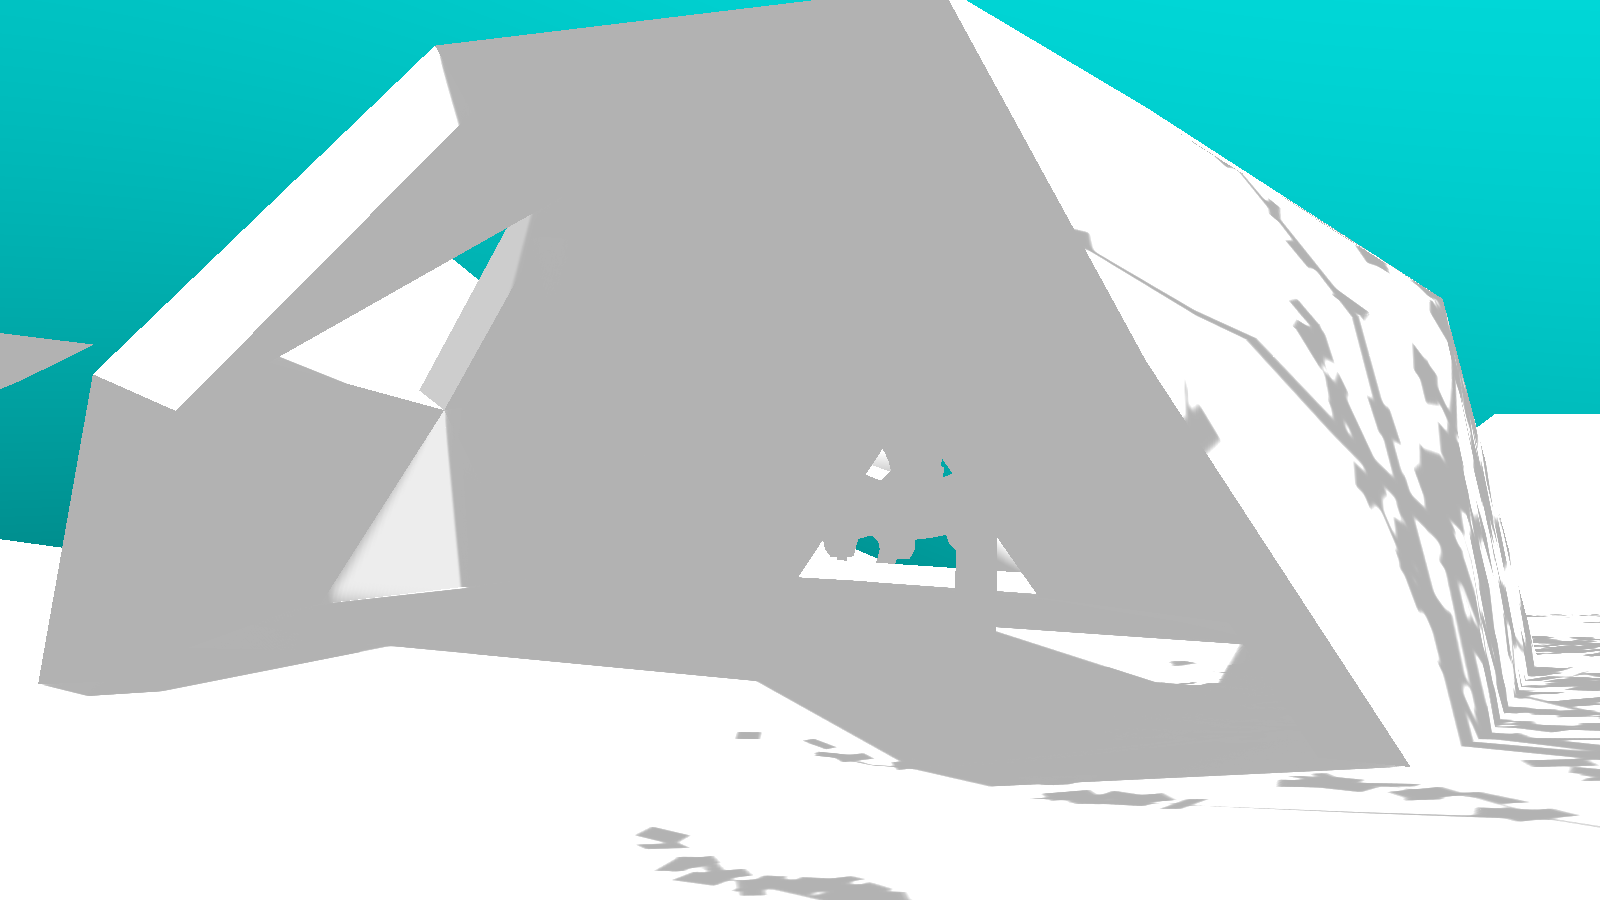
\includegraphics[width = 5.5cm]{vo_assets/presentaton_graphics/dome/plainResult.png}
		\label{ref:plainRendering}
	}\quad\quad
	\centering
	\subfloat[Rendering mit ASVO: Zahnräder sind sichtbar]
	{

		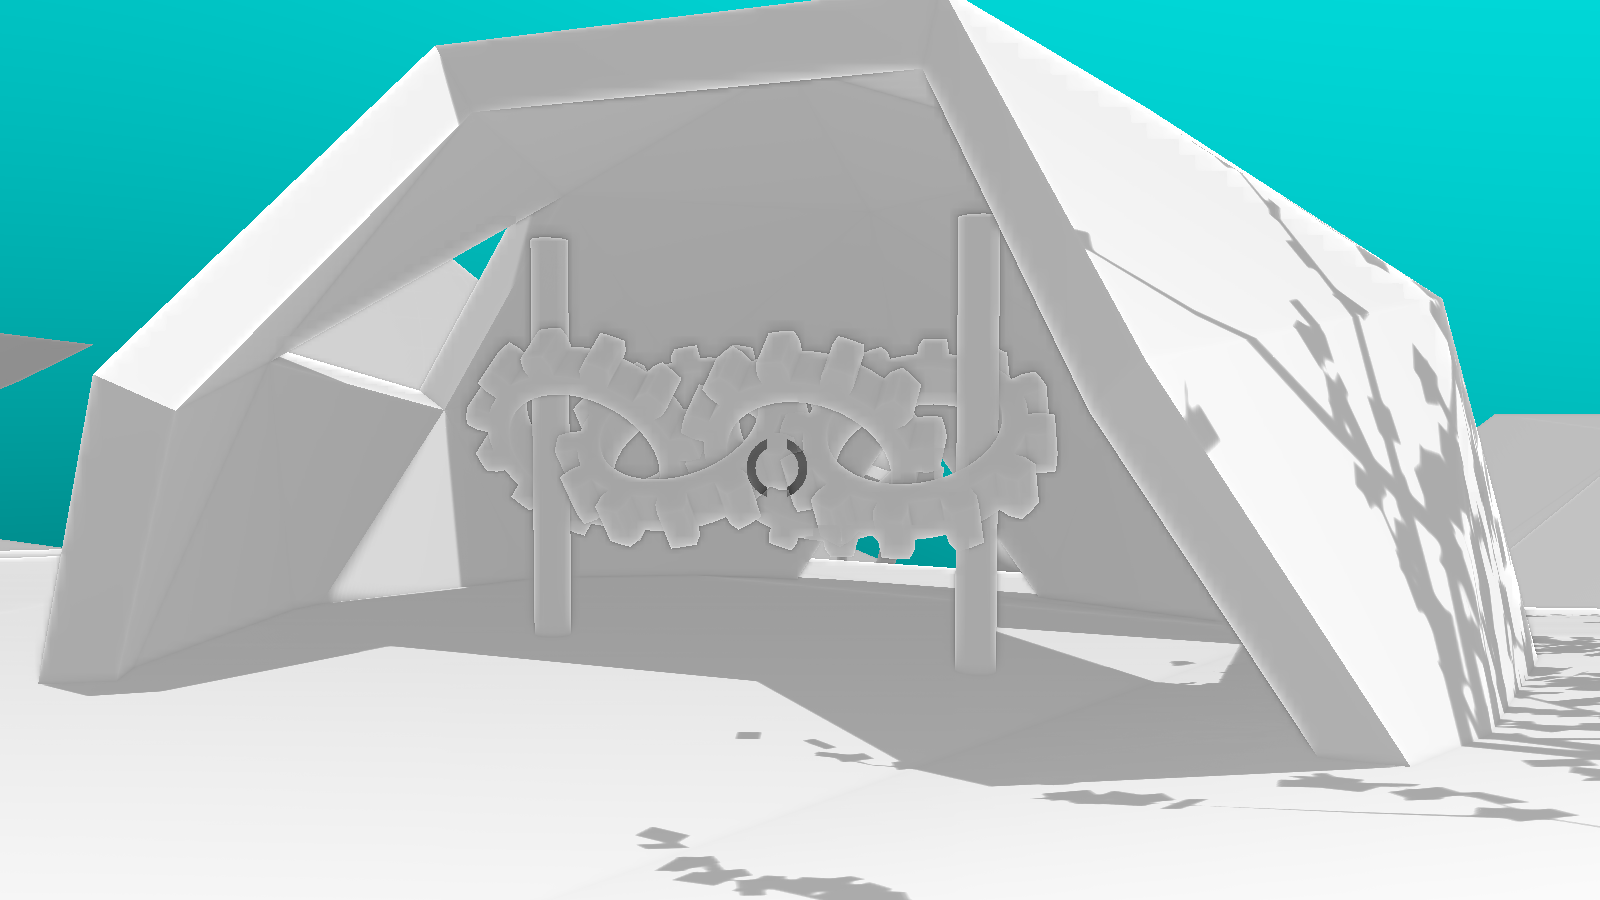
\includegraphics[width = 5.5cm]{vo_assets/presentaton_graphics/dome/ASVO.png}
		\label{ref:ASVORendering}
	}
	\caption{Scene mit und ohne VO}
	\label{ref:finalVO}
\end{figure}
Durch die Approximierung durch Mipmaps sind jedoch bei
großflächiger Filterung durch Area Sampled Volumetric Obscurance mehr Artefakte zu sehen. Hier bietet es sich an in Zukunft noch alternative
Mipmap-Filtertechniken auszuprobieren um diese Artefakte zu vermeiden. Unsere Technik mit Binomialem
Filtering über die Mipmap-Ebenen eliminiert zwar schon eine große Anzahl an Artefakten, vollkommen
Artefaktfrei ist das ergebnis jedoch noch nicht, hier können in Zukunft vielleicht noch bessere Ergebnisse
erzielt werden, in dem die Filter noch optimiert werden.

% Fazit
\subsection{Moment Shadow Mapping}
Das Moment Shadow Mapping bietet uns Schatten mit hoher Qualität, welche auch sehr gut zur Geltung kommen. Artefakte wie Aliasing und Light Leaking werden stärker gemindert als bei VSM möglich. Ausserdem funktionierte die Implementierung sehr einfach durch den gegeben HLSL Code. Das Verfahren ist schnell und bietet beim Filtern viele Freiheiten. Wir nutzen Gauss und 1xMSAA-16xMSAA welches verschiedene Ergebnisse liefert.

\begin{figure}[H]
	\centering
	\subfloat[Gauss Filter]{

		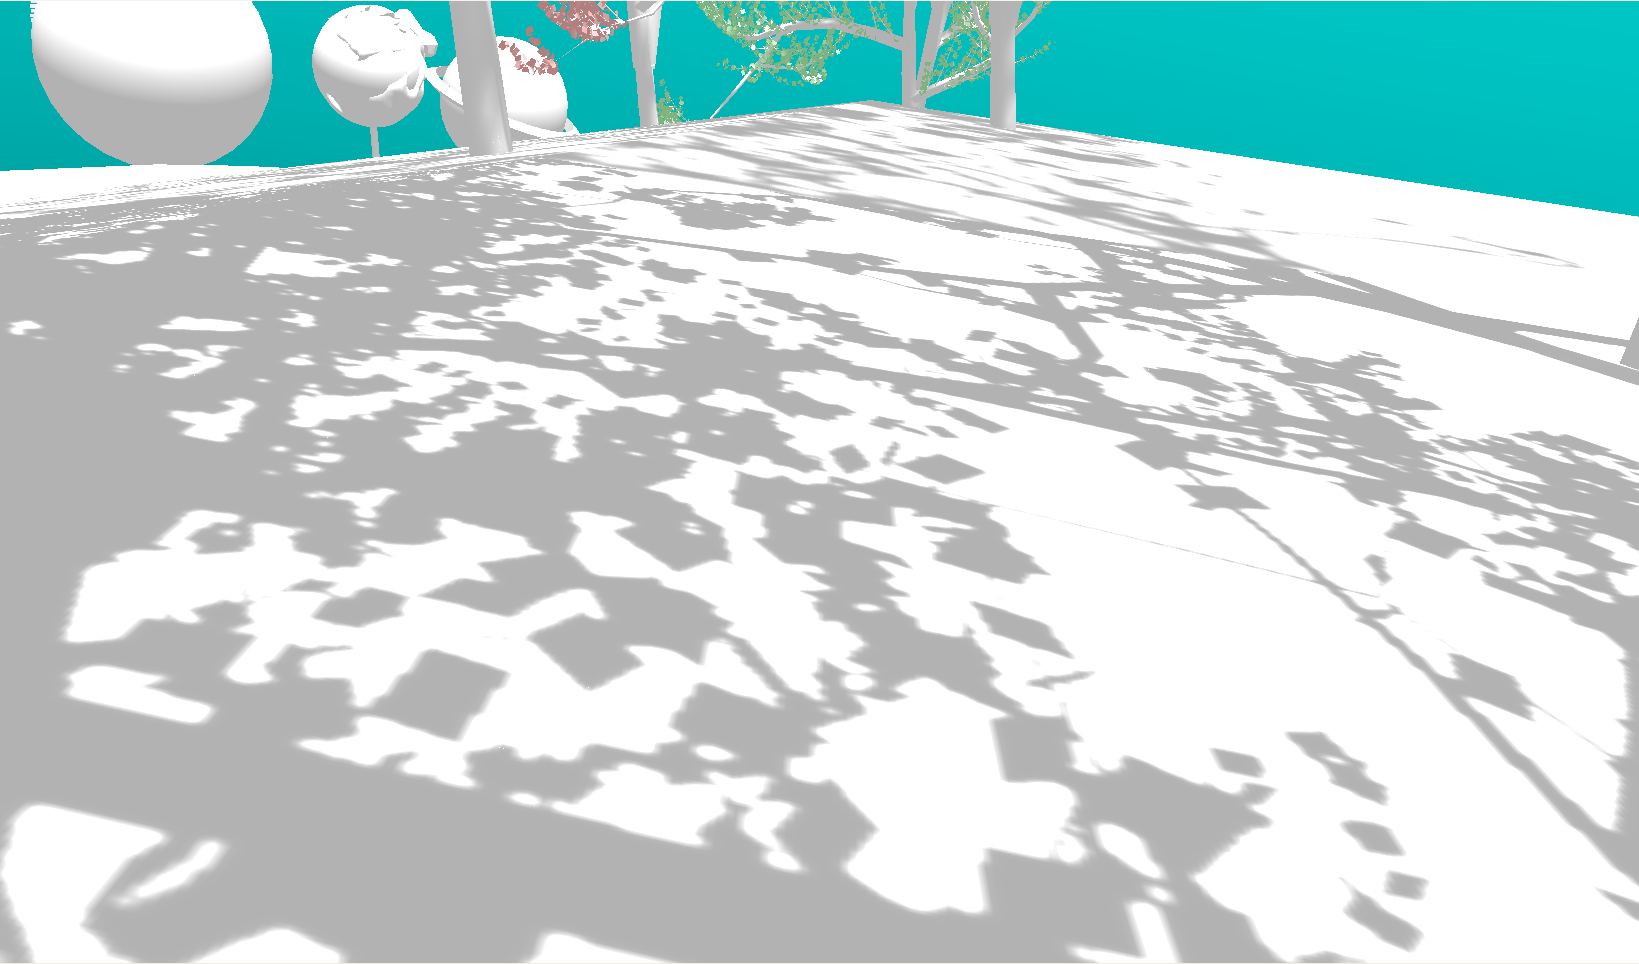
\includegraphics[width = 6cm]{msm_assets/baumGauss.png}
		\label{ref:msmgauss}
	}
    \subfloat[1xMSAA]{

		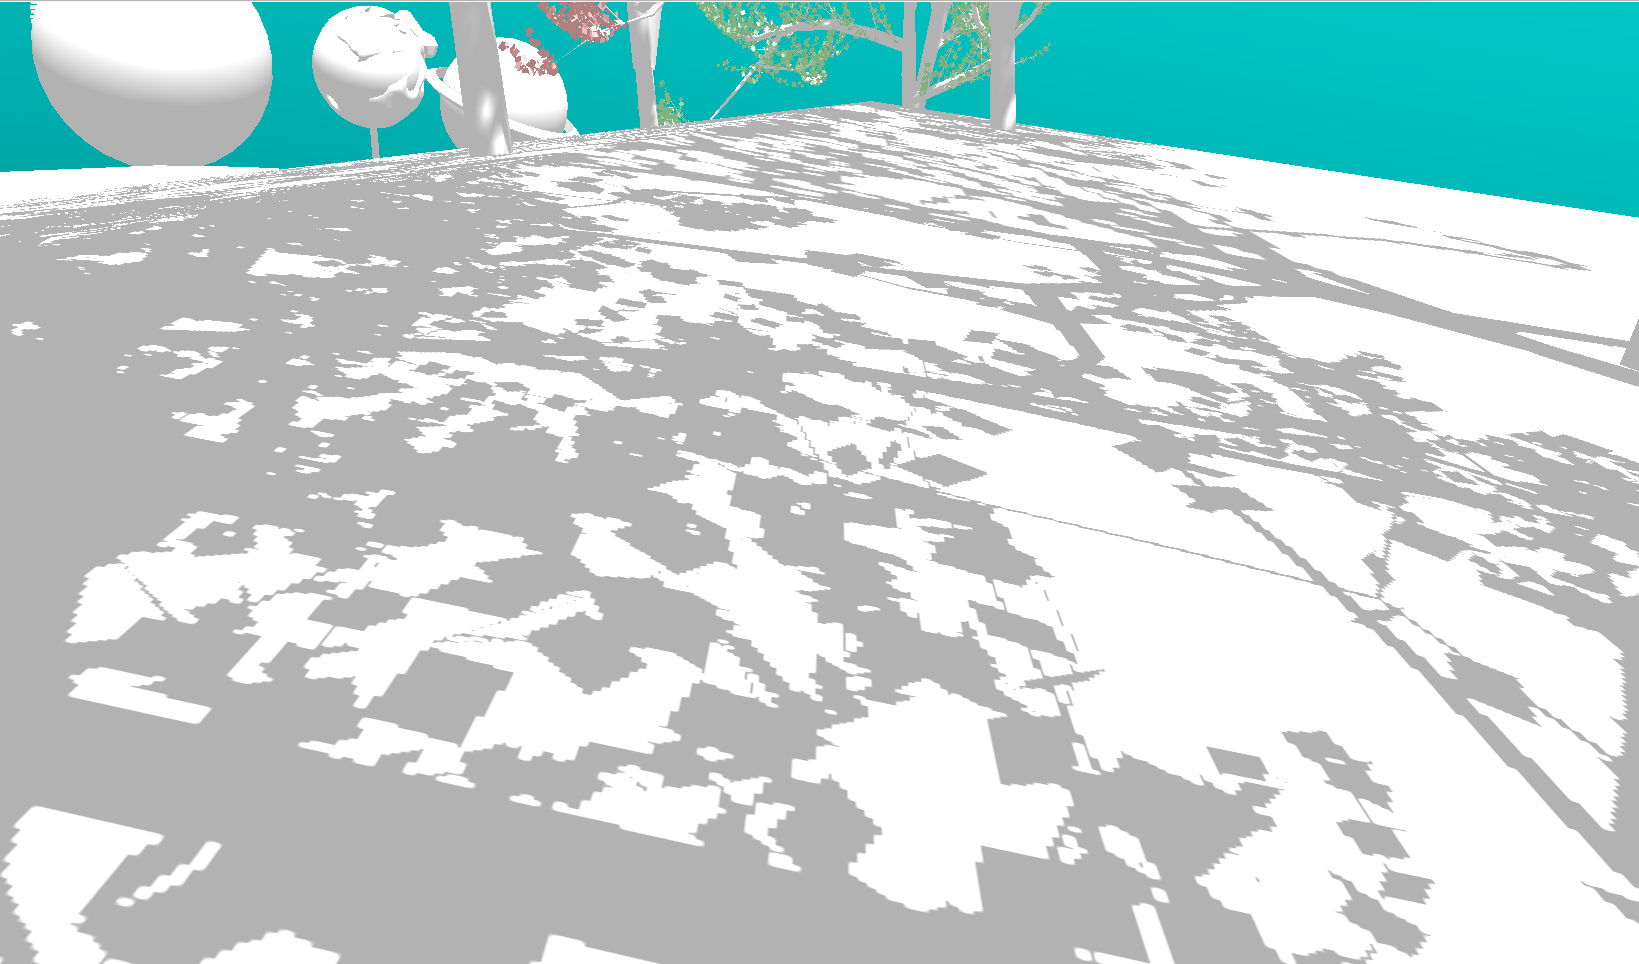
\includegraphics[width = 6cm]{msm_assets/baum1MSAA.png}
		\label{ref:msm1}
	}
	
	\subfloat[2xMSAA]{
		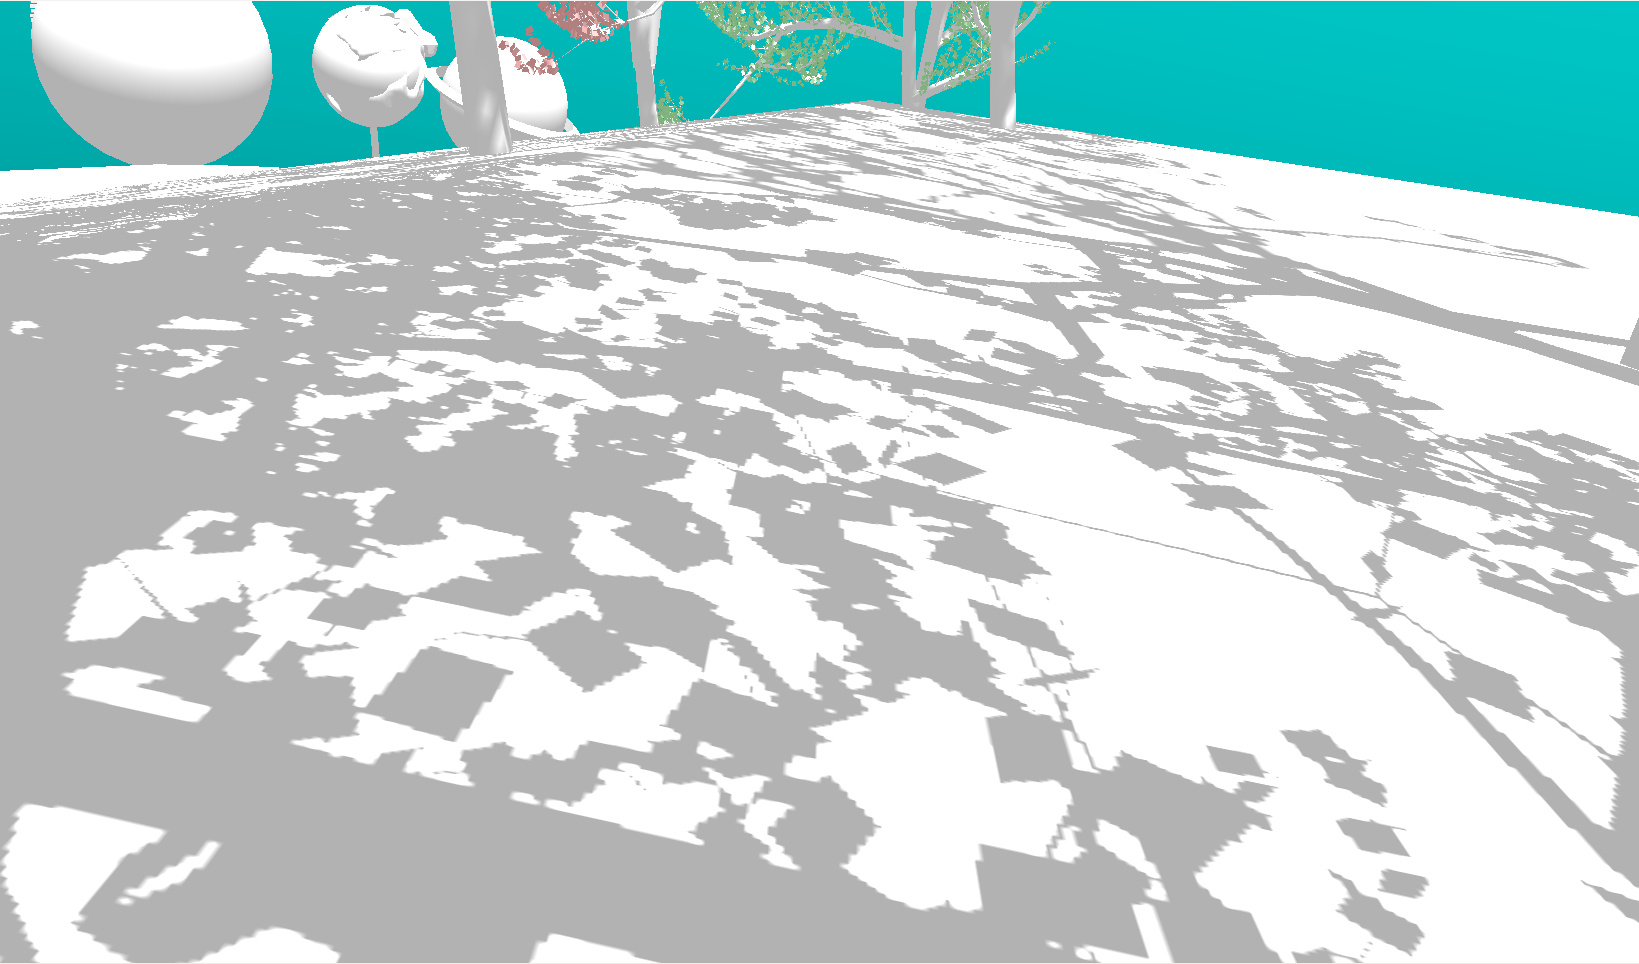
\includegraphics[width = 6cm]{msm_assets/baum2MSAA.png}
		\label{ref:msm2}
	}
	\subfloat[16xMSAA]{
		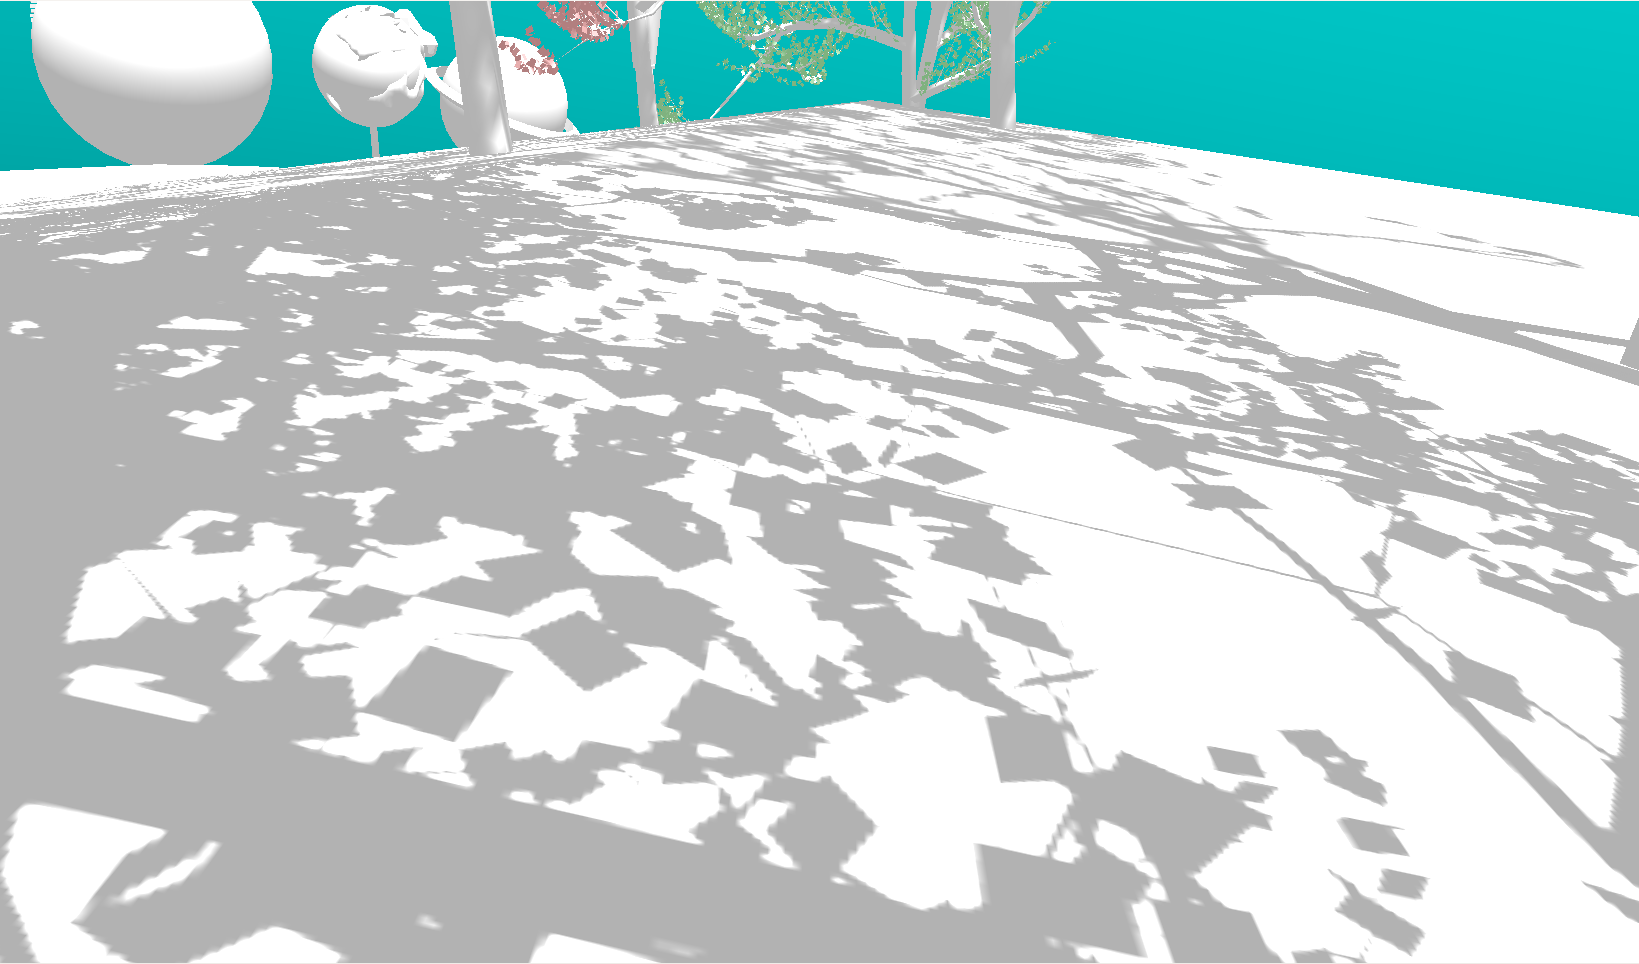
\includegraphics[width = 6cm]{msm_assets/baum16MSAA.png}
		\label{ref:msm16}
	}
	\caption{Moment Shadow Mapping mit Gauss Filter, 1xMSAA bis 16x MSAA. Hierbei ist zu beachten das 1xMSAA zwischen Pixeln interpoliert}
\end{figure}

Auch dies hat sich kaum auf die Performance ausgewirkt und wir sind mit dem Ergebniss sehr zufrieden.
Im direkten Verlgleich zu PCF fällt auf, das MSM weitere Artefakte unterbindet. Im Verlgleich zu VSM bieten die 4 statt 2 Momente ebenfalls einen Vorteil. Light Leaking wird effektiv vermindert, was bei VSM nicht der Fall ist.
Für die Zukunft wollen wir noch weiteres Filtern testen sowie weiter vermindern.

Auch wenn MSM und SDSM zunächst wie orthogonale Verfahren aussehen, beeinflusst die variable Größe der Shadow Maps einer Kaskade die Filterbarkeit mit Gauss.
Um eine gewisse Filter Größe der Shadow Map im Screen Space zu erreichen, muss die Shadow Map mit einer variablen Standardabweichung $\sigma$ gefiltert werden.
Da die Shadow Map Frusta teilweise sehr kleine Bereiche abdecken werden die Filtermasken sehr groß.
Mip-Mapping hat dieses Problem nicht.


% Fazit
\subsection{Moment Based Volumetric Obscurance}
\begin{figure}[H]
	\centering
	\subfloat[MBVO Beispiel 1]{

		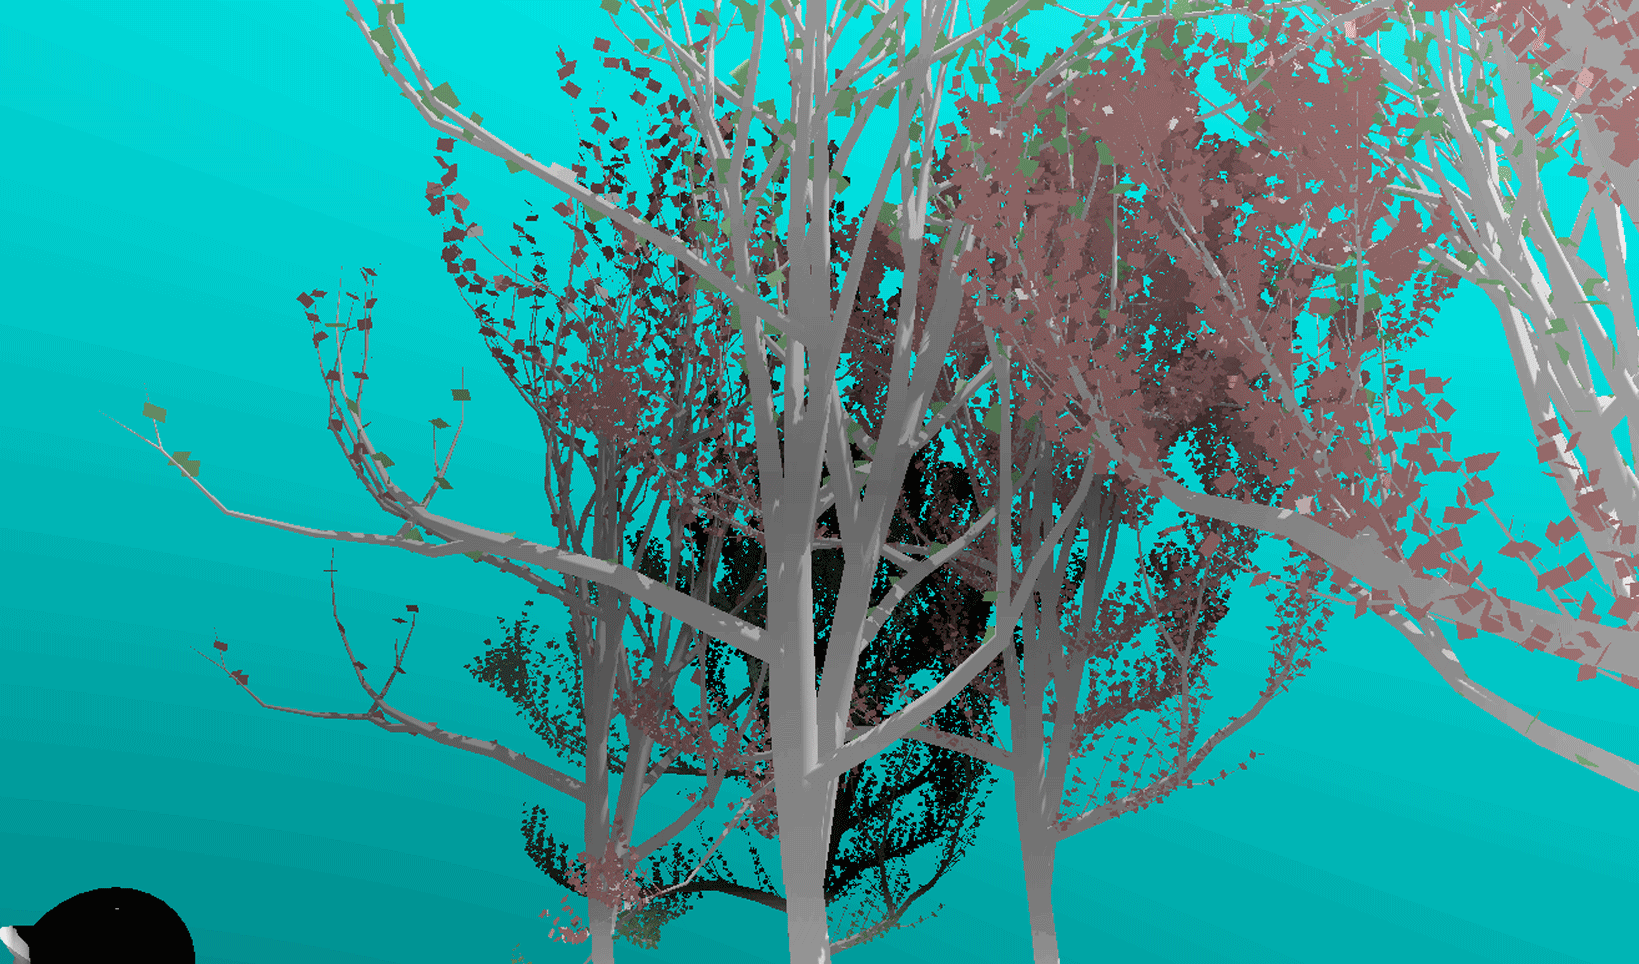
\includegraphics[width = 6cm]{msm_assets/mbvo/scene_with_mvbo2.png}
		\label{ref:mbvo1}
	}
    \subfloat[MBVO Beispiel 2]{

		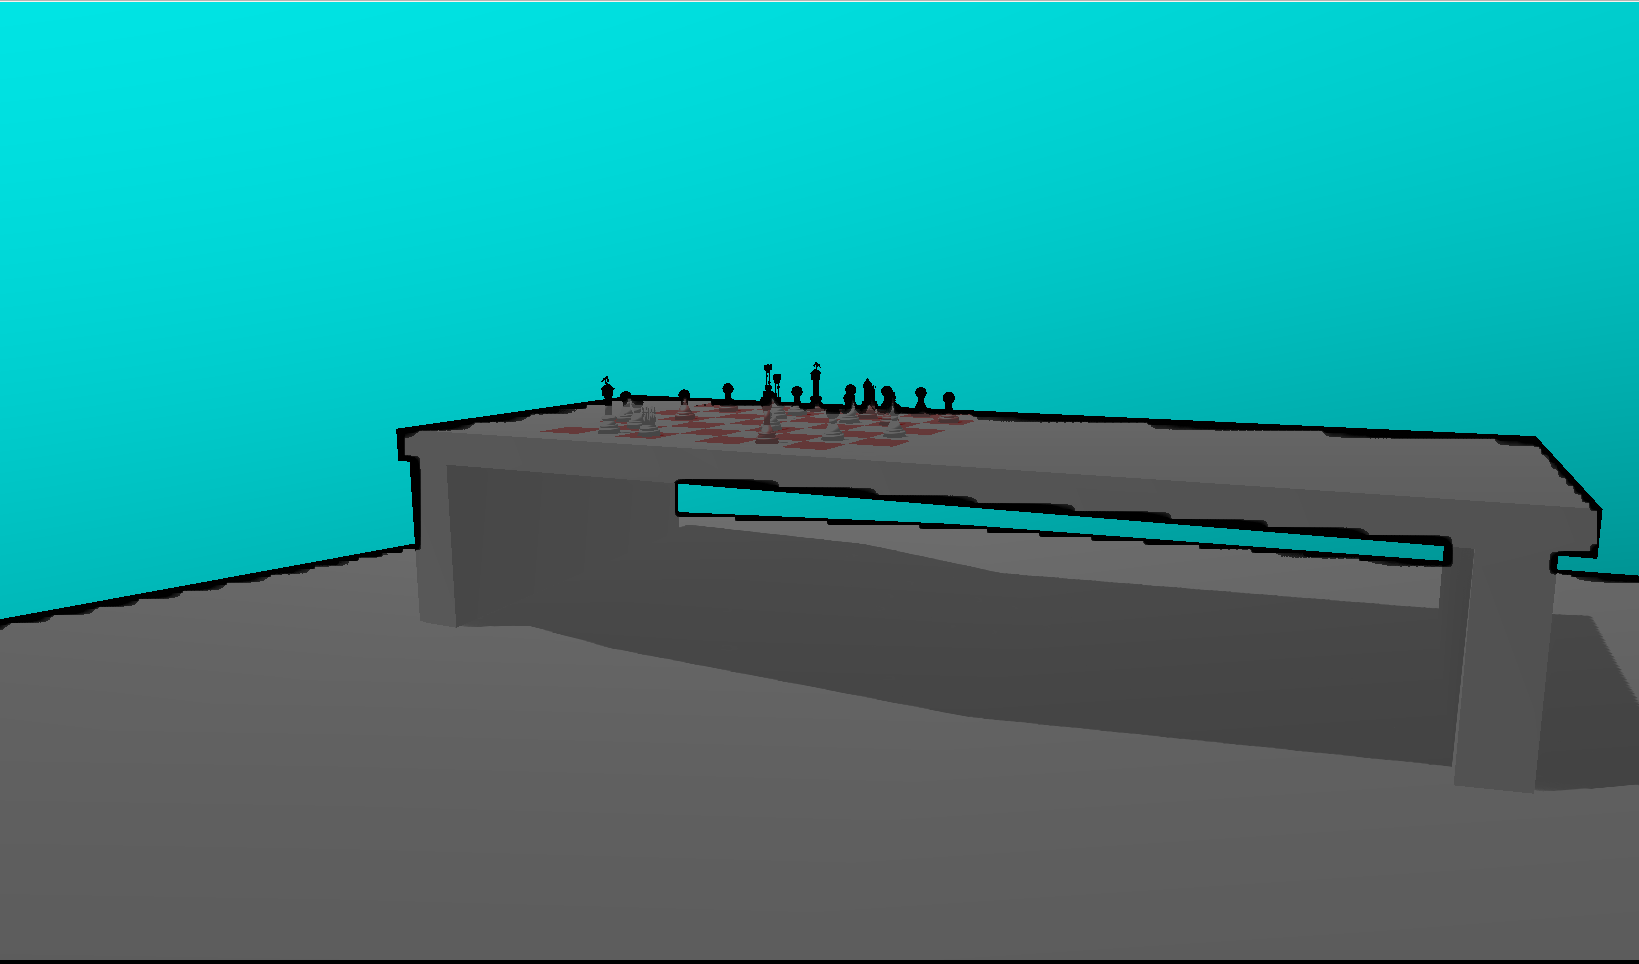
\includegraphics[width = 6cm]{msm_assets/mbvo002.png}
		\label{ref:mbvo2}
	}
	
	\subfloat[MBVO Beispiel 2]{
		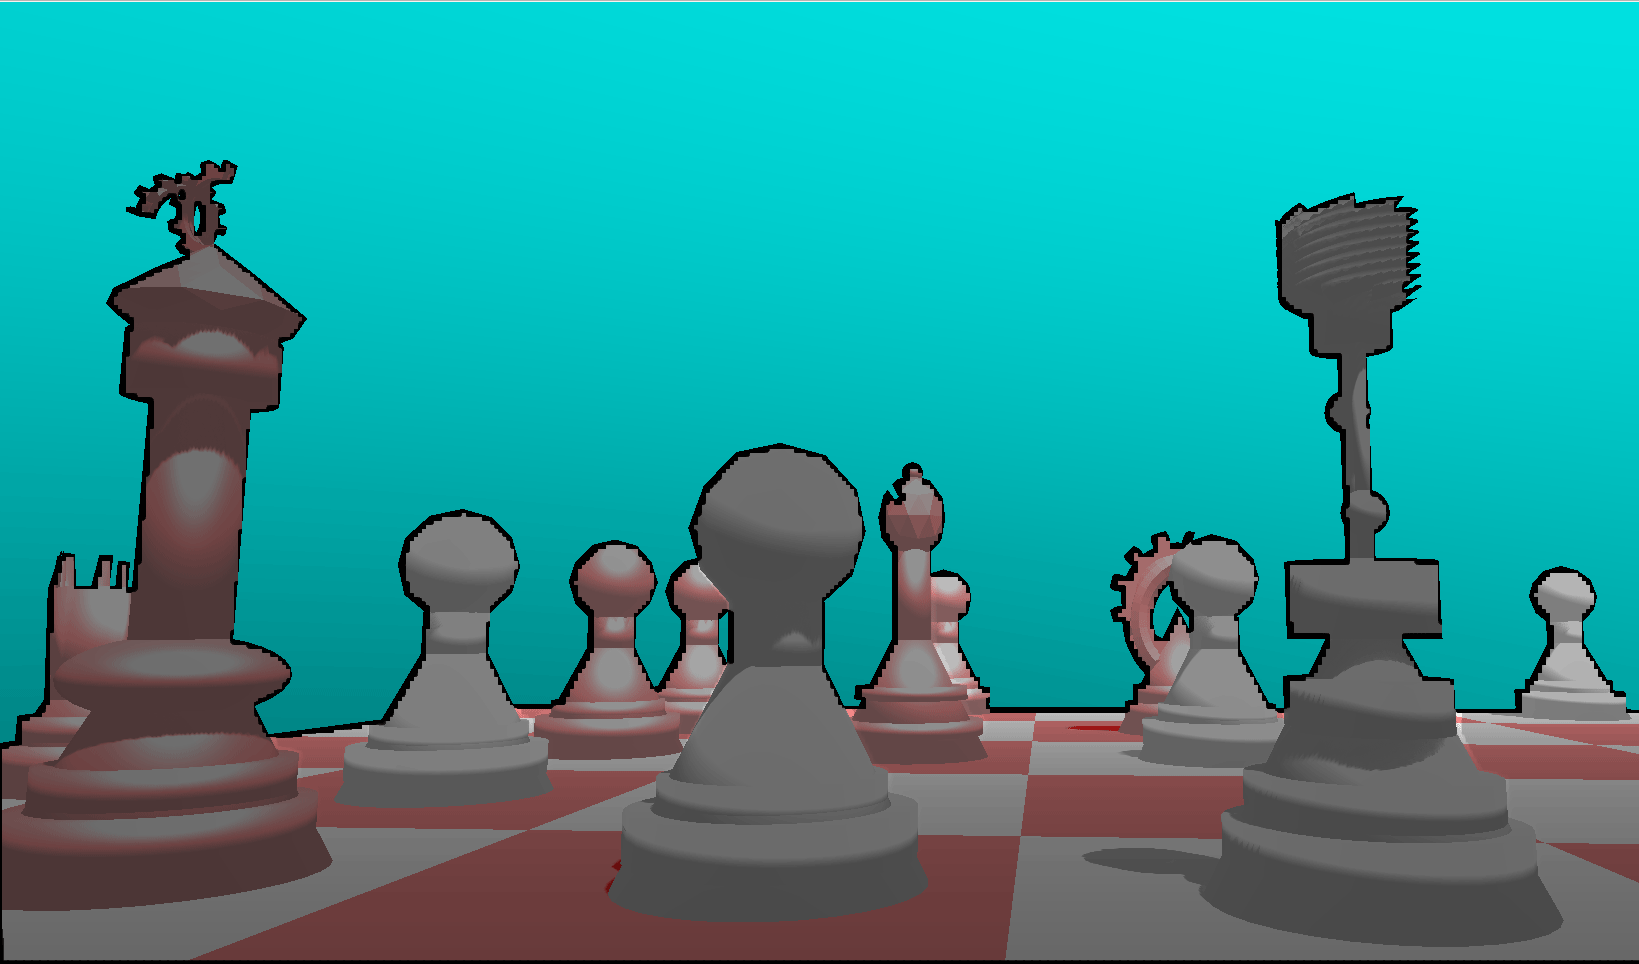
\includegraphics[width = 6cm]{msm_assets/mbvo003.png}
		\label{ref:mbvo3}
	}
	\subfloat[MBVO Beispiel 3]{
		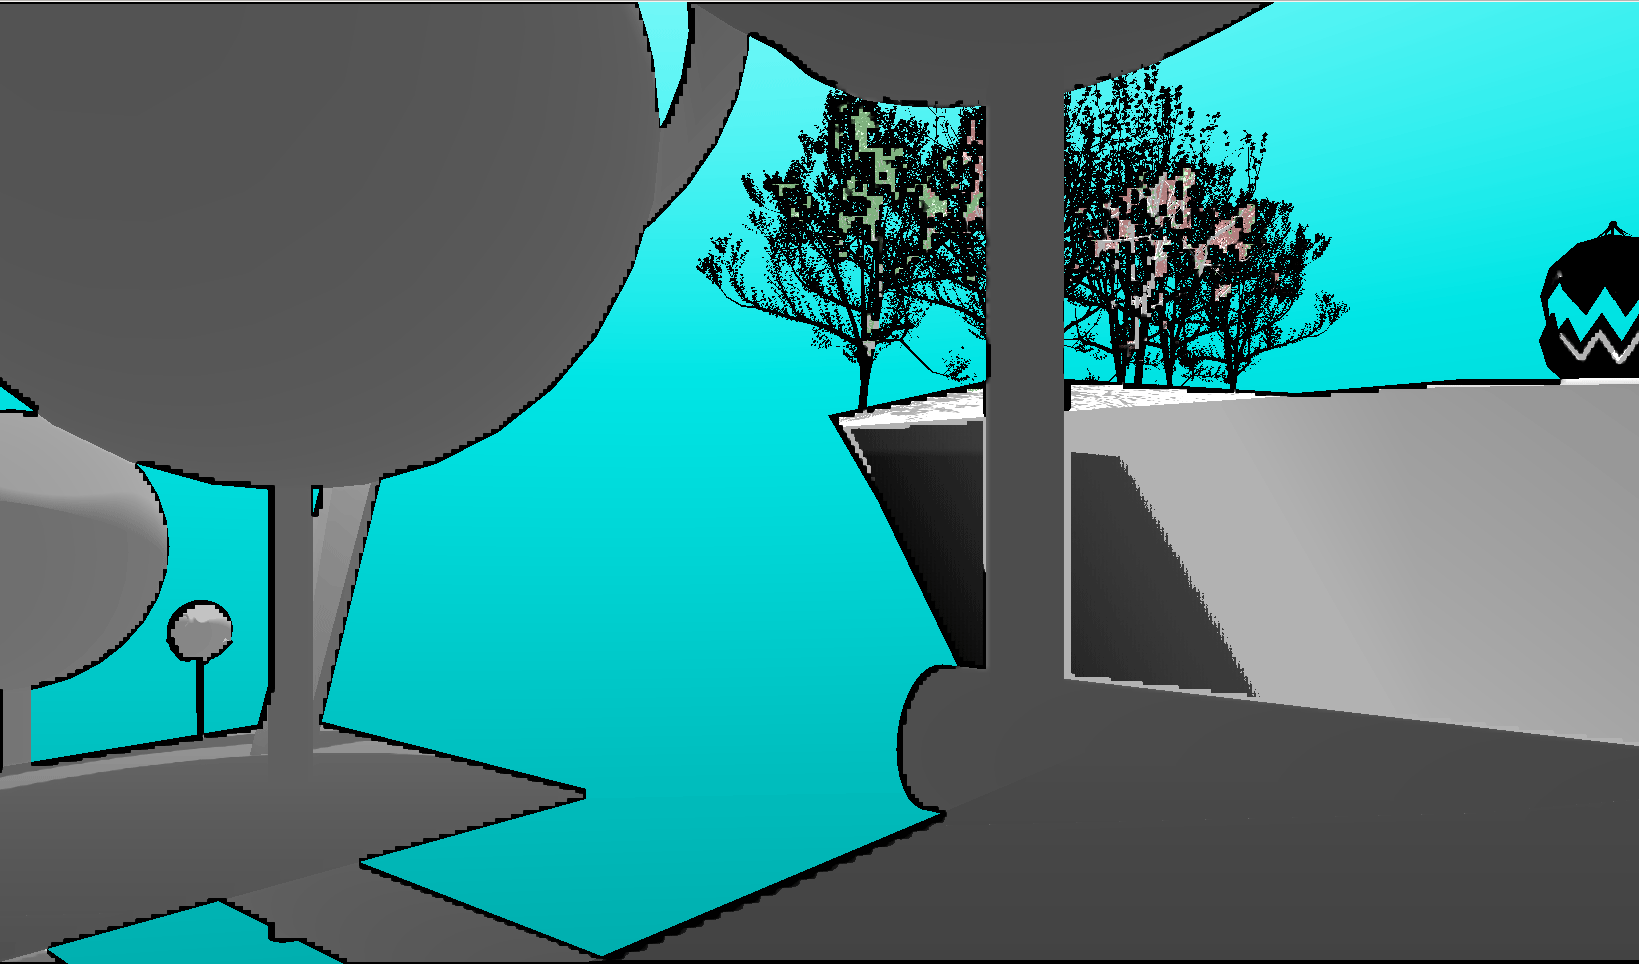
\includegraphics[width = 6cm]{msm_assets/mbvo004.png}
		\label{ref:mbvo4}
	}
	\caption{Moment Based Volumetric Obscurance Beispiele mit verschiedenen Geometrien und Entfernungen}
\end{figure}

Das Verfahren zur Moment Based Volumetric Obscurance war ebenfalls leicht umzusetzen, da sich die Implementierung kaum vom MSM unterscheidet. Das Verfahren bietet ein ästethisches Bild mit sehr wenig Rauschen. Es ähnelt dem Volumetric Obscurance mit Area Sampling.

% Literaturverzeichnis:
\bibliography{lit}
\bibliographystyle{alpha}

\end{document}

